\documentclass[landscape,twocolumn,letter]{book}
% Licencia y derechos: consulte ../../LICENSE-CC-BY-4.0.
% Las figuras y demás materiales de terceros pueden tener derechos separados y deben identificarse.

\usepackage[spanish]{babel}
\usepackage[left=1.5cm, right=1.5cm, top=1.5cm, bottom=1.5cm]{geometry}

\usepackage{hyperref}
\usepackage{graphicx}
\usepackage{caption}
\usepackage{subcaption}
\usepackage{setspace}
\usepackage{fancyhdr}
\usepackage{mathtools}

\DeclareCaptionLabelSeparator{emdash}{\textemdash}
\captionsetup[figure]{labelsep=emdash,font=onehalfspacing,position=bottom}
\captionsetup{%
	singlelinecheck=off,
	skip=2pt,
	justification=centering,
}

\makeindex 

\title{Apuntes de Electrónica I}
\date{2026 Noviembre\\rev 0.1}
\author{Alberto Medrano\thanks{Instructor, Universidad de Los Andes (ULA)}}
\begin{document}
	\pagestyle{fancy}
	
	\fancyhead{} % clear all header fields
	\fancyhead[RO,LE]{\textbf{Apuntes del Instructor:} Electrónica I}
	\fancyfoot{} % clear all footer fields
	\fancyfoot[LE,RO]{\thepage}
	\fancyfoot[LO,CE]{Compilado por: A. Medrano}
	
	\maketitle

	\noindent\small
	\textbf{Licencia:} Este material derivado del libro del Profesor Oscar Fuentes se distribuye bajo
	\href{https://creativecommons.org/licenses/by/4.0/deed.es}{CC BY 4.0}.
	Cualquier figura o material de terceros conserva sus derechos y licencia propios y debe identificarse por separado.

	
\includegraphics[width=0.4\linewidth]{_fig/ULA.pdf}
	
	\textbf{Sobre el contenido de éstos apuntes}

	- - -

	Ésto es una remasterización del libro del Profesor Oscar Fuentes. De encontrar algún error o sugerencia por favor notificar vía correo electrónico a \href{mailto: medrano.alberto@ula.ve}{medrano.alberto@ula.ve}

	- - -

	Agradecimiento especial a los alumnos para con la transcripción del contenido:

	\begin{itemize}
		\item \textbf{2026-B:} Angel Osorio, Jesús Ramírez y Mitzael Rivas por las páginas digitalizadas durante su curso en la asignatura Electrónica I.
	\end{itemize}

	\tableofcontents
	
    % Licencia y derechos: consulte ../../LICENSE-CC-BY-4.0.
% Las figuras y demás materiales de terceros pueden tener derechos separados y deben identificarse.

\chapter{Amplificador operacional}

Las señales eléctricas generadas por los diversos tipos de transductores tienen, por lo general, magnitudes demasiado pequeñas para producir efectos físicos útiles. En la mayor parte de los casos es necesario amplificar dichas señales antes de intentar utilizarlas en el control de procesos, la transmisión y procesamiento de información, etc. En este capítulo se estudia las características y formas de uso del amplificador operacional, uno de los dispositivos más frecuentemente utilizados para construir circuitos capaces de amplificar señales.

\section{Generalidades}
El amplificador operacional es un dispositivo con una estructura interna bastante compleja. Sin embargo, su funcionamiento es relativamente fácil de describir y, a través de esta descripción, es posible presentar en forma simple los conceptos fundamentales que son comunes a todo tipo de amplificadores.

\subsection{Símbolo}
El símbolo de un amplificador operacional se muestra en la figura \ref{fig:op-amp_gen_simbolo}. El dispositivo posee dos entradas: entrada no inversora ($+$) y entrada inversora ($-$). La señal fluye de izquierda a derecha, en la dirección de la punta de flecha, desde una o ambas entradas hacia el terminal de salida.

\begin{figure}[h]
	\centering
	\subfloat[Símbolo]
	{
		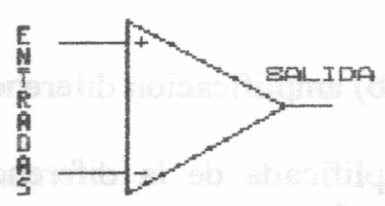
\includegraphics[width=0.4\linewidth]{_fig/op-amp_gen_simbolo.png}
		\label{fig:op-amp_gen_simbolo}
	}
	\subfloat[Polarización]
	{
		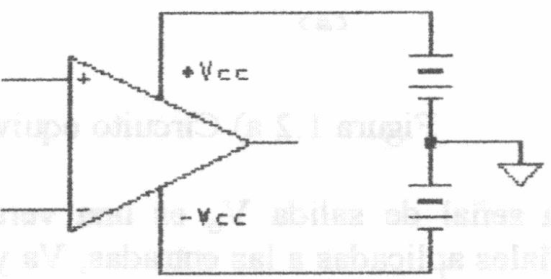
\includegraphics[width=0.4\linewidth]{_fig/op-amp_gen_polarizacion.png}
		\label{fig:op-amp_gen_polarizacion}
	}
	\caption{Amplificador operacional}
	\label{fig:op-amp_gen}
\end{figure}

Los terminales identificados con $+V_{cc}$ y $-V_{cc}$ permiten inyectar corriente continua al amplificador operacional desde fuentes de tensión según el esquema mostrado en la figura \ref{fig:op-amp_gen_polarizacion}. Estas corrientes, llamadas de polarización, son necesarias para el funcionamiento del amplificador y puede considerarse que el dispositivo convierte una fracción de la potencia continua proveniente desde las fuentes de polarización en potencia alterna o de señal. Todos los amplificadores operacionales deben ser polarizados para que puedan funcionar. Generalmente, y con el propósito de simplificar los diagramas, se omiten en éstos los terminales de polarización.

\subsection{Modelo simple}
Un amplificador operacional tiene una estructura interna bastante compleja. Sin embargo, desde el punto de vista de su funcionamiento eléctrico y en aplicaciones simples puede ser representado como equivalente al circuito mostrado dentro del bloque dibujado con línea segmentada en la figura \ref{_fig:op-amp_simple_eq}. Esto es, en una primera aproximación, un amplificador operacional se comporta como un circuito capaz de amplificar linealmente la diferencia entre las señales aplicadas a sus entradas.

\begin{figure}[h]
	\centering
	\subfloat[Circuito equivalente]
	{
		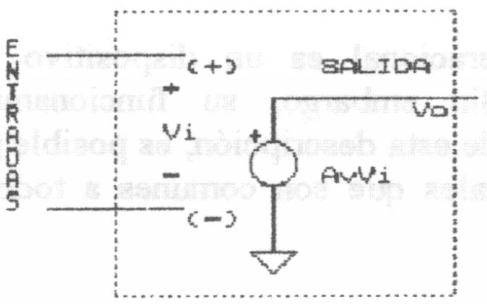
\includegraphics[width=0.4\linewidth]{_fig/op-amp_simple_eq.png}
		\label{fig:op-amp_simple_eq}
	}
	\subfloat[Amplificador diferencial]
	{
		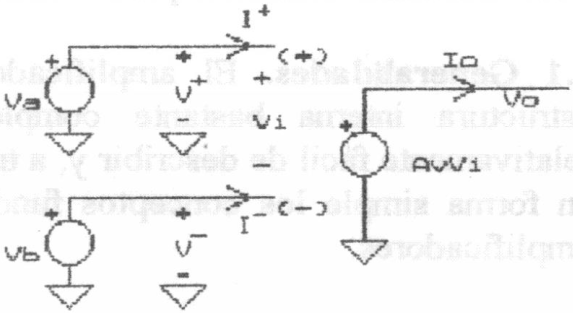
\includegraphics[width=0.4\linewidth]{_fig/op-amp_simple_diff.png}
		\label{fig:op-amp_simple_diff}
	}
	\caption{Modelo simple}
	\label{fig:op-amp_simple}
\end{figure}

La señal de salida $V_O$ es una versión amplificada de la diferencia entre las señales aplicadas a las entradas, $V_a$ y $V_b$. En efecto,

\begin{equation}
	Vo = Av * (V^+ - V^-) = Av * Vi \quad ; \quad Vi = V^+ - V^-
\end{equation}

\begin{equation}
	V^+ = Va \quad ; \quad V^- = Vb \quad ; \quad Vo = Av * (Va - Vb)
\end{equation}

En la ecuación anterior, $Av$ es la llamada ganancia diferencial del amplificador operacional y $V^+$ y $V^-$ son las tensiones, referidas a tierra, de las entradas no inversora e inversora, respectivamente.

En el circuito equivalente simplificado de la figura anterior se observa que las corrientes en las entradas, $I^+$ e $I^-$, serán siempre cero pues dichas entradas están internamente conectadas a circuitos abiertos. En cambio, la corriente en el terminal de salida dependerá de los elementos conectados externamente a este terminal y, generalmente será diferente de cero.

\section{Amplificador operacional ideal}
Se dice que el amplificador operacional es ideal si, en el modelo de la figura \ref{fig:op-amp_simple_diff}, la ganancia diferencial $Av$ tiende a infinito. El análisis de circuitos que contienen amplificadores operacionales ideales es, por lo general, muy simple y produce, en muchos casos, resultados que se aproximan razonablemente a los resultados observados en circuitos reales.

\begin{figure}[h]
	\centering
	\subfloat[Amplificador inversor]
	{
		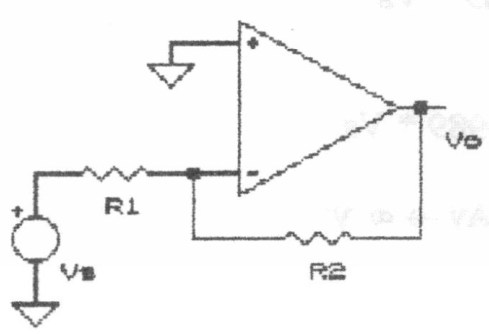
\includegraphics[width=0.4\linewidth]{_fig/op-amp_inversor_sch.png}
		\label{fig:op-amp_inversor_sch}
	}
	\subfloat[Circuito equivalente]
	{
		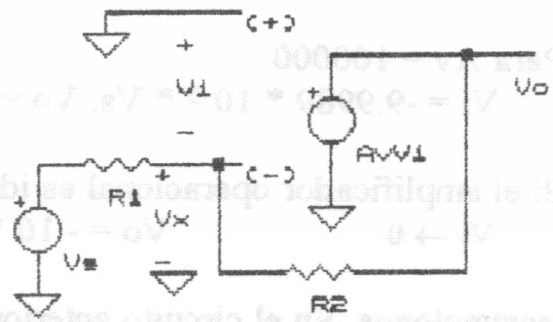
\includegraphics[width=0.4\linewidth]{_fig/op-amp_inversor_eq.png}
		\label{fig:op-amp_inversor_eq}
	}
	\caption{Amplificador operacional ideal}
	\label{fig:op-amp_inversor}
\end{figure}

\textbf{Ejemplo.} En el circuito de la figura \ref{fig:op-amp_inversor}, $R_1 = 1\text{ K}$; $R_2 = 10\text{ K}$. Hallar la expresión de $Vo$ usando el modelo simple. Considerar a) $Av = 10000$; b) $Av = 100000$; c) $Av = \infty$ (amplificador operacional ideal).

En la figura \ref{fig:op-amp_inversor_eq}, el amplificador operacional ha sido reemplazado por el modelo simple de la figura \ref{fig:op-amp_simple_eq}. Aplicando el teorema de Millman para determinar $Vx = -Vi$ se tiene:

\begin{equation}
	V^- = Vx = -Vi = \frac{\dfrac{Vs}{R_1} + \dfrac{AvVi}{R_2}}{\dfrac{1}{R_1} + \dfrac{1}{R_2}}
\end{equation}

Despejando $Vi$:

\begin{equation}
	Vi = \frac{-Vs}{\left(1 + (1 + Av) * \dfrac{R_1}{R_2}\right)}
\end{equation}

Además, $Vo = Av * Vi$:

\begin{equation}
	Vo = \frac{- Av * Vs}{(1 + (1 + Av) * \dfrac{R_1}{R_2})}
\end{equation}

\textbf{a) Con $Av = 10000$, puede encontrarse:}
$$Vi = -9.989 * 10^{-4} * Vs, \quad Vo = -9.989 * Vs$$

\textbf{b) Para $Av = 100000$:}
$$Vi = -9.9989 * 10^{-5} * Vs, \quad Vo = -9.9989 * Vs$$

\textbf{c) Si el amplificador operacional es ideal, $Av \to \infty$ y:}
$$Vi \to 0 \qquad \qquad Vo = - 10 * Vs$$

\textbf{Observaciones.} En el circuito anterior:

\begin{enumerate}
	\item En las expresiones de $Vi$ y $Vo$, el signo - indica que estas tensiones están opuestas en fase respecto a $Vs$. Esto es, si $Vs$ aumenta, $Vo$ disminuirá y viceversa. El amplificador anterior invierte la fase y de allí su nombre de \textbf{amplificador inversor}.
	\item La magnitud de $Vi$ disminuye al aumentar la magnitud de $Av$. En el caso del amplificador operacional ideal ($Av \to \infty$), $Vi \to 0$ y la tensión en la entrada inversora, $V^+$, se hace igual a la tensión en la entrada no inversora, $V^-$. Se dice que las entradas forman un nodo "virtual", esto es que ambas entradas tienen la misma tensión sin estar conectadas entre sí. Esta situación es típica de circuitos con amplificadores operacionales ideales en los que exista realimentación negativa, esto es, circuitos en los que algún elemento esté conectado entre la salida y la entrada inversora.
	\item Si se considera, como ocurre en la realidad, que el amplificador operacional tiene una ganancia finita, el valor elevado de ésta asegura que la ganancia teórica del circuito difiere muy poco de la ganancia "ideal". Por ejemplo, para $Av = 100000$, la diferencia es de 1 parte en 1000, bastante menor que la tolerancia de las resistencias usadas en aplicaciones simples. En estos casos simples, la ganancia ideal será una aproximación razonable a la ganancia real.
\end{enumerate}

\subsection{Análisis de Circuitos con amplificadores operacionales ideales}
En un circuito con realimentación negativa, implementado con un amplificador operacional ideal, puede usarse la relación $Vi = 0$ para encontrar en forma directa la tensión de salida. Ver figura \ref{fig:op-amp_inversor-ideal}.

\begin{figure}[h]
	\centering
	\subfloat[Ideal]
	{
		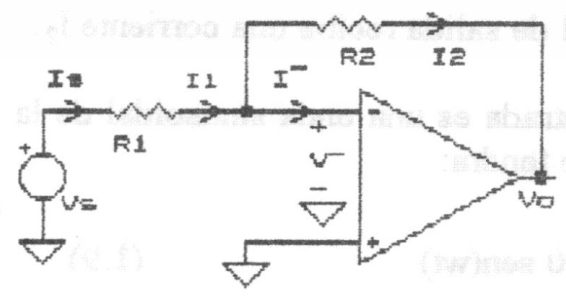
\includegraphics[width=0.4\linewidth]{_fig/op-amp_inversor-ideal_sch.png}
		\label{fig:op-amp_inversor-ideal_sch}
	}
	\subfloat[Señales]
	{
		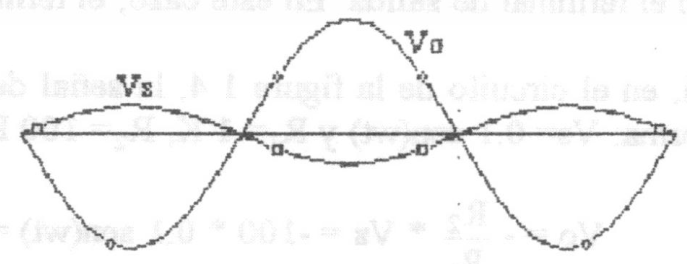
\includegraphics[width=0.4\linewidth]{_fig/op-amp_inversor-ideal_senales.png}
		\label{fig:op-amp_inversor-ideal_senales}
	}
	\caption{Amplificador operacional inversor}
	\label{fig:op-amp_inversor-ideal}
\end{figure}

\subsubsection{Amplificador inversor}
El circuito anterior tiene realimentación negativa (en este caso, a través de $R_2$) e incluye un amplificador operacional ideal ($Av \to \infty$). En estas condiciones, la tensión entre las entradas es $Vi = V^+ - V^- = 0$. Además, $V^+ = 0$ puesto que la entrada no inversora está conectada a tierra.

Así:

\begin{equation}
	V^- = V^+ = 0
\end{equation}

La corriente $I_1$ estará dada por:

\begin{equation}
	I_1 = \frac{Vs - V^-}{R_1} = \frac{Vs}{R_1} = I_2 + I^- = I_2 \text{ pues } I^- = 0
\end{equation}

La tensión de salida es:

\begin{equation}
	Vo = V^- - I_2 * R_2 = 0 - I_2 * R_2 = - \frac{R_2}{R_1} * Vs
\end{equation}

\begin{description}
	\item[Ganancia de tensión, $K$:] Se define ganancia de tensión del circuito a la relación $Vo/Vs$ que llamaremos $K$. En este circuito, $K = - R_2/R_1$. El signo - indica que la señal de salida estará invertida (desfasada $180^\circ$), respecto de la señal de entrada.
	\item[Impedancia de entrada, $Z_i$:] Se llama impedancia de entrada $Zi$ a: $Zi = Vs/Is$. La impedancia de entrada, como su nombre lo indica, corresponde al valor de impedancia que, conectado a $Vs$, tomaría de esta fuente la misma corriente $Is$ que el circuito original. En el circuito anterior, $Is = I_1 = Vs/R_1$. De aquí, $Zi = R_1$. Es importante destacar, una vez más, que a pesar de que la corriente en las entradas del amplificador operacional es cero, no ocurre lo mismo con la corriente en el terminal de salida. En este caso, el terminal de salida recibe una corriente $I_2$.
\end{description}

Si, en el circuito de la figura 1.4, la señal de entrada es una onda sinusoidal de la forma: $Vs = 0.1 \text{ sen}(wt)$ y $R_1 = 1\text{ K}$, $R_2 = 100\text{ K}$ se tendrá:

\begin{equation}
	Vo = - \frac{R_2}{R_1} * Vs = -100 * 0.1 \text{ sen}(wt) = -10 \text{ sen}(wt)
\end{equation}

La impedancia de entrada será $Zi = R_1 = 1\text{ K}$. Por su parte, la corriente $I_2$ entra al terminal de salida y estará dada por:

\begin{equation}
	I_2 = I_2 = \frac{Vs}{R_1} = 100 \text{ sen}(wt) \text{ uA}
\end{equation}

Se observa que la corriente en el terminal de salida es diferente de cero.

\subsubsection{Amplificador no inversor}
El circuito de un amplificador no inversor se muestra en la figura \ref{fig:op-amp_n-inversor-ideal}.

\begin{figure}[h]
	\centering
	\subfloat[Ideal]
	{
		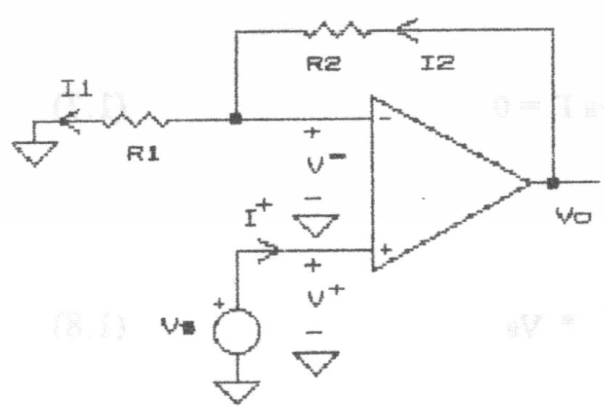
\includegraphics[width=0.4\linewidth]{_fig/op-amp_n-inversor-ideal_sch.png}
		\label{fig:op-amp_n-inversor-ideal_sch}
	}
	\subfloat[Señales]
	{
		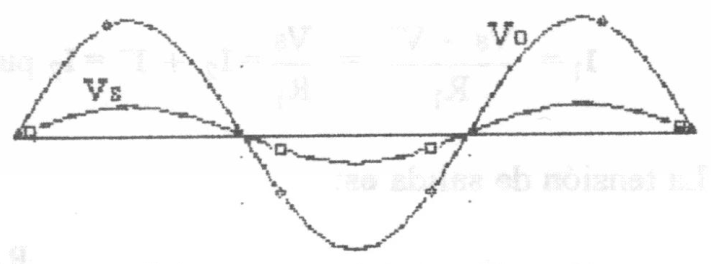
\includegraphics[width=0.4\linewidth]{_fig/op-amp_n-inversor-ideal_senales.png}
		\label{fig:op-amp_n-inversor-ideal_senales}
	}
	\caption{Amplificador operacional no inversor}
	\label{fig:op-amp_n-inversor-ideal}
\end{figure}

En el circuito anterior $Vi = 0$, esto es, la tensión de salida se ajustará a un valor tal que $V^-$ iguale a $V^+$. Además, la corriente en la entrada inversora, $I^+$, es cero. Así, tenemos:

\begin{equation}
	V^- = V^+ = Vs
\end{equation}

\begin{equation}
	I_1 = \frac{Vs}{R_1} = I_2 = \frac{Vo - V^-}{R_2} = \frac{Vo - Vs}{R_2}
\end{equation}

Puede despejarse:

\begin{equation}
	Vo = \left(1 + \frac{R_2}{R_1}\right) * Vs
\end{equation}

La señal de salida tiene la misma fase que la señal de entrada. Para este circuito, la ganancia $K = Vo/Vs$ es:

\begin{equation}
	K = \frac{Vo}{Vs} = 1 + \frac{R_2}{R_1}
\end{equation}

En este circuito, la señal de entrada está conectada directamente a la entrada no inversora. Puesto que esta entrada no toma corriente ($Is = 0$), la impedancia de entrada de este circuito es:

\begin{equation}
	Zi = \frac{Vs}{Is} = \infty
\end{equation}

Si $R_1 = 1\text{ K}$; $R_2 = 9\text{ K}$ y $Vs = 1\text{ sen}(wt)\text{ volt}$, la tensión de salida será:

\begin{equation}
	Vo = \left(1 + \frac{R_2}{R_1}\right) * Vs = 10\text{ sen}(wt)
\end{equation}

La corriente $I_2$ sale del terminal de salida y tiene un valor de:

\begin{equation}
	I_2 = I_1 = \frac{Vs}{R_1} = \frac{Vo - V^-}{R_2} = 1\text{ sen}(wt)\text{ mA}
\end{equation}

\subsubsection{Seguidor de tensión}
Idealmente, el circuito de la figura \ref{fig:op-amp_seguidor}, caso especial del amplificador no inversor ($R_1 = \infty$; $R_2 = 0$), tiene una impedancia de entrada infinita. En este circuito, la señal de salida $Vo$ es idéntica a la señal de entrada $Vs$. Por esta razón se le llama seguidor de voltaje.

\begin{figure}[h]
	\centering
	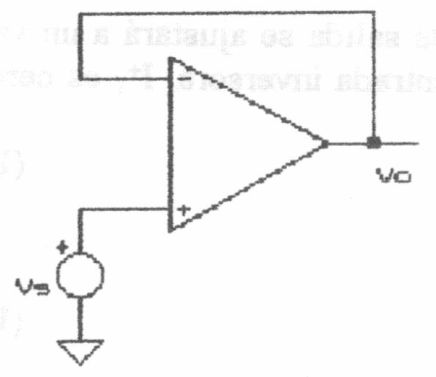
\includegraphics[width=0.6\linewidth]{_fig/op-amp_seguidor.png}
	\caption{Seguidor de voltaje}
	\label{fig:op-amp_seguidor}
\end{figure}

\subsubsection{Amplificador diferencial}
La señal de salida del circuito de la figura \ref{fig:op-amp_diff} es proporcional a la diferencia entre las señales de entrada $V_1$ y $V_2$.

\begin{figure}[h]
	\centering
	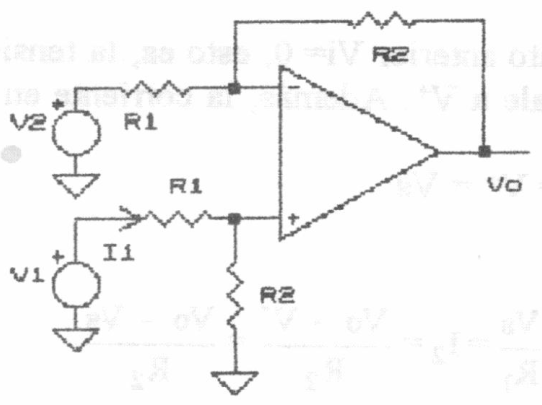
\includegraphics[width=0.6\linewidth]{_fig/op-amp_diff.png}
	\caption{Seguidor de voltaje}
	\label{fig:op-amp_diff}
\end{figure}

Aplicando superposición se tiene:

\textbf{a) $V_1 \neq 0$, $V_2 = 0$.} Para la señal $V^+$, el circuito se comporta como un amplificador no inversor:

\begin{equation}
	Vo' = \left(1 + \frac{R_2}{R_1}\right) * V^+ = \left(1 + \frac{R_2}{R_1}\right) * \frac{V_1 * R_2}{(R_1 + R_2)}
\end{equation}

\begin{equation}
	Vo' = \frac{R_2}{R_1} * V_1
\end{equation}

\textbf{b) $V_1 = 0$, $V_2 \neq 0$.} El circuito se comporta un amplificador inversor para la señal $V_2$. La red resistiva conectada a la entrada no inversora no tiene efecto.

\begin{equation}
	Vo'' = - \frac{R_2}{R_1} * V_2
\end{equation}

Así,

\begin{equation}
	Vo = Vo' + Vo'' = \frac{R_2}{R_1} * (V_1 - V_2)
\end{equation}

La ganancia diferencial del circuito es $Vo / (V_1 - V_2) = R_2 / R_1$. Esta ganancia no debe confundirse con la ganancia diferencial del amplificador operacional, $Av = Vo / Vi$. La impedancia de entrada debe determinarse en el circuito original de la figura 1.6b. La impedancia vista desde la fuente $V_1$ es:

\begin{equation}
	Zi(V_1) = V_1 / I_1 = V_1 / I_1 = R_1 + R_2
\end{equation}

En cambio, la corriente que entrega la fuente $V_2$ depende del valor de $V_1$. Por lo tanto, no es procedente definir una impedancia de entrada para la fuente $V_2$.

\textbf{Señal de entrada flotante, $Vd$.} Si el amplificador diferencial tiene aplicada una señal $Vd$ que no está referida a tierra (señal de entrada flotante) la estructura del circuito corresponderá a la mostrada en la figura \ref{fig:op-amp_diffb_float}.

\begin{figure}[h]
	\centering
	\subfloat[Con señal entrada flotante]
	{
		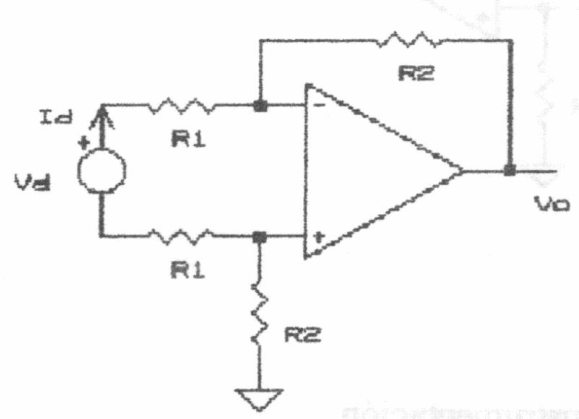
\includegraphics[width=0.4\linewidth]{_fig/op-amp_diffb_float.png}
		\label{fig:op-amp_diffb_float}
	}
	\subfloat[con señal de entrada de modo común]
	{
		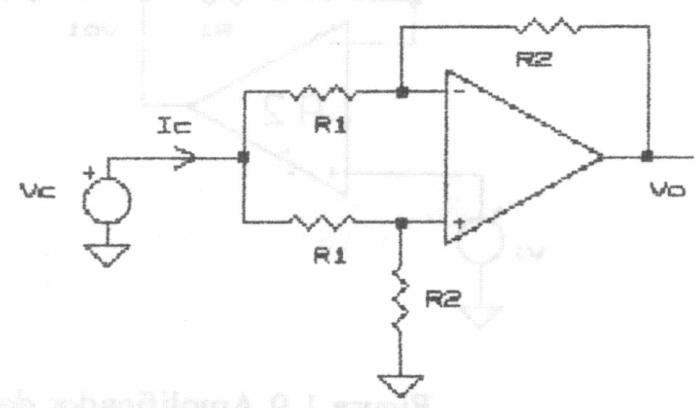
\includegraphics[width=0.4\linewidth]{_fig/op-amp_diffb_comun.png}
		\label{fig:op-amp_diffb_comun}
	}
	\caption{Amplificador diferencial}
	\label{fig:op-amp_diffb}
\end{figure}

En este circuito se cumple que:

\begin{equation}
	Id = \frac{Vd}{2 R_1}; \quad \text{además,} \quad Vo = - \frac{R_2}{R_1} * Vd
\end{equation}

En este caso, la impedancia de entrada $Zi$ es:

\begin{equation}
	Zi = \frac{Vd}{Id} = 2 R_1
\end{equation}

\textbf{Señal de entrada de modo común, $Vc$.} Si una señal de entrada se aplica simultáneamente a ambas entradas del amplificador diferencial, se dice que dicha señal es una señal de modo común. En esta situación, descrita en la figura 1.8b, la señal de salida es cero. La impedancia de entrada vista desde $Vc$ es:

\begin{equation}
	Zi = \frac{Vc}{Ic} = \frac{R_1 + R_2}{2}
\end{equation}

\begin{figure}[h]
	\centering
	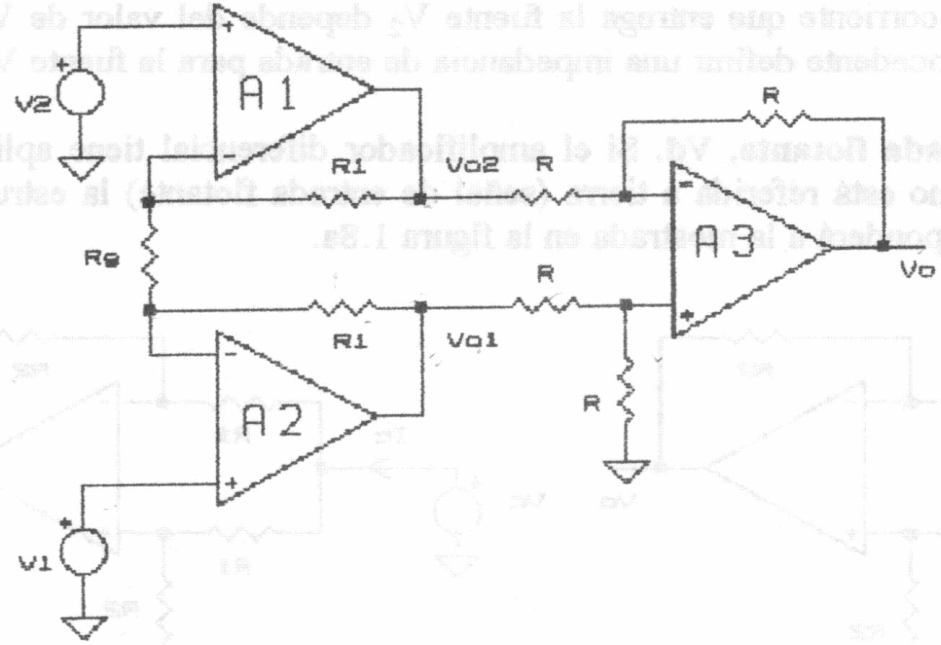
\includegraphics[width=0.6\linewidth]{_fig/op-amp_instru.png}
	\caption{Amplificador de instrumentación}
	\label{fig:op-amp_instru}
\end{figure}

\subsubsection{Amplificador de instrumentación}
El circuito de la figura 1.9 presenta una impedancia de entrada muy alta (idealmente infinita) y una señal de salida que depende únicamente de la diferencia entre las señales de entrada $V_1$ y $V_2$. Estas características son deseables cuando se desea amplificar señales pequeñas en presencia de ruido o señales generadas por sensores con impedancias internas elevadas o que varían en el tiempo.

La primera etapa formada por $A1$ y $A2$ presenta una impedancia de entrada muy elevada (idealmente infinita) a las fuentes $V_1$ y $V_2$. Las señales de salida $Vo_1$ y $Vo_2$ están dadas por:

\begin{equation}
	Vo_1 = \left(1 + \frac{R_1}{Rg}\right) * V_1 - \frac{R_1}{Rg} * V_2
\end{equation}

\begin{equation}
	Vo_2 = - \frac{R_1}{Rg} * V_1 + \left(1 + \frac{R_1}{Rg}\right) * V_2
\end{equation}

La etapa final es un amplificador diferencial con ganancia unitaria. La señal de salida total es:

\begin{equation}
	Vo = Vo_1 - Vo_2 = (V_1 - V_2) * \left(1 + \frac{2 R_1}{Rg}\right)
\end{equation}

Esto es, la señal de salida depende únicamente de la diferencia entre las señales de entrada. Es posible demostrar que este circuito exhibe este comportamiento aún cuando las resistencias de la etapa de entrada sean diferentes. En versiones integradas del amplificador diferencial, la ganancia se controla externamente mediante $Rg$.

\subsubsection{Integrador y derivador}
El circuito de la figura \ref{fig:op-amp_integrador} puede integrar señales analógicas:

\begin{figure}[h]
	\centering
	\subfloat[Integrador]
	{
		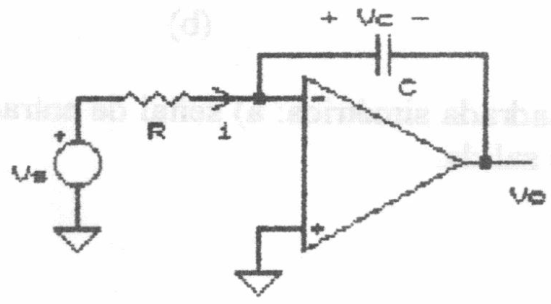
\includegraphics[width=0.4\linewidth]{_fig/op-amp_integrador.png}
		\label{fig:op-amp_integrador}
	}
	\subfloat[Derivador]
	{
		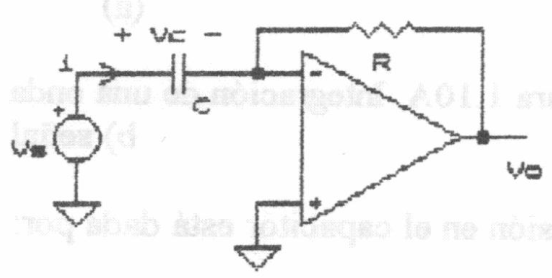
\includegraphics[width=0.4\linewidth]{_fig/op-amp_derivador.png}
		\label{fig:op-amp_derivador}
	}
	\caption{Configuraciones}
	\label{fig:op-amp_integrador-derivador}
\end{figure}

\begin{equation}
	i = \frac{Vs}{R}
\end{equation}

\begin{equation}
	Vo = - Vcap = - \frac{1}{C} \int i \, dt = - \frac{1}{RC} \int Vs \, dt
\end{equation}

En cambio, en el circuito de la figura \ref{fig:op-amp_derivador}:

\begin{equation}
	i = C \frac{dV_s}{dt}
\end{equation}

\begin{equation}
	Vo = - i * R = - RC * \frac{dV_s}{dt}
\end{equation}

Esto es, la señal de salida es proporcional a la derivada de la señal de entrada.

\textbf{Ejemplo.} En el circuito integrador de la figura \ref{fig:op-amp_ejm1a} hallar $Vo$. $C$ está inicialmente descargado. Hallar $Vo(t)$.

\begin{figure}[h]
	\centering
	\subfloat[Señal del entrada]
	{
		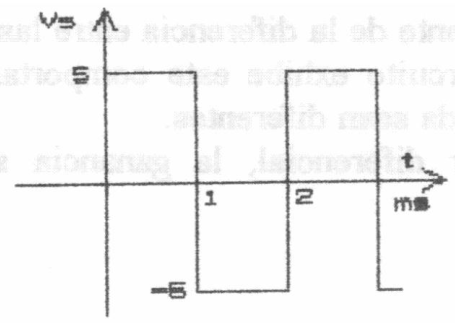
\includegraphics[width=0.4\linewidth]{_fig/op-amp_ejm1a.png}
		\label{fig:op-amp_ejm1a}
	}
	\subfloat[Señal de salida]
	{
		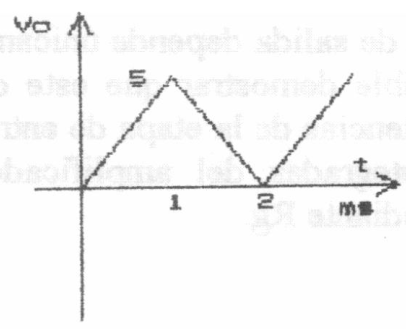
\includegraphics[width=0.4\linewidth]{_fig/op-amp_ejm1b.png}
		\label{fig:op-amp_ejm1b}
	}
	\caption{Integración de una onda cuadrada simétrica}
	\label{fig:op-amp_ejm1}
\end{figure}

La tensión en el capacitor está dada por:

\begin{equation}
	Vc(t) = \frac{1}{RC} \int Vs \, dt + Vc(\text{inicial})
\end{equation}

Por su parte, la tensión de salida del circuito es:
\begin{equation}
	Vo(t) = - Vc(t)
\end{equation}

\textbf{Intervalo 0-1ms:} $C$ está descargado en $t = 0$ por lo que la tensión de salida en este intervalo es:

\begin{equation}
	Vc(t) = \frac{1}{RC} \int_{0}^{t} Vs \, dt + Vc(\text{inicial}) = \frac{1}{10^3 * 10^{-6}} \int_{0}^{t} 5 \, dt + 0 = 5000 \, t
\end{equation}

esto es:
\begin{equation}
	Vo(t) = - Vc(t) = - 5000 \, t
\end{equation}

al término del intervalo:
\begin{equation}
	Vo(t = 1\text{ ms}) = - Vc(t = 1\text{ ms}) = - 5000 \, (10^{-3}) = -5
\end{equation}

La tensión en $C$ al término de este intervalo, ($5\text{ volt}$), es el valor inicial de $Vc$ para el intervalo siguiente.

\textbf{intervalo 1-2 ms:} En este intervalo $Vs = -5$. Ahora la expresión de la tensión en $C$ es:

\begin{equation}
	Vc(t) = \frac{1}{RC} \int_{1\text{ ms}}^{t} Vs \, dt + Vc(\text{inicial}) = \frac{1}{10^3 * 10^{-6}} \int_{1\text{ ms}}^{t} (-5) \, dt + 5 = -5000 \, (t - 1\text{ ms}) + 5
\end{equation}

Al término del intervalo:
\begin{equation}
	Vc(t = 2\text{ ms}) = 0
\end{equation}

La tensión de salida es:
\begin{equation}
	Vo(t) = - Vc(t) = 5000 \, (t - 1\text{ ms}) - 5
\end{equation}

Se observa que la tensión de salida al término de este intervalo es $0\text{ volt}$. El circuito tendrá, a partir de $2\text{ ms}$, una respuesta periódica.

\begin{figure}[h]
	\centering
	\subfloat[Circuito integrador]
	{
		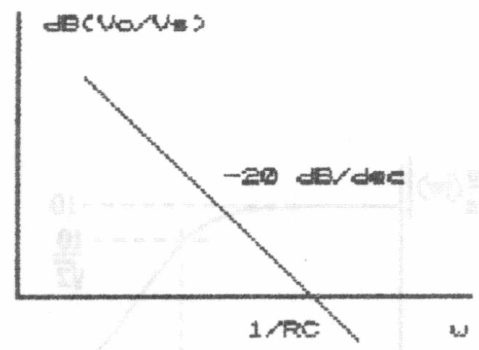
\includegraphics[width=0.4\linewidth]{_fig/op-amp_ejm1a_bode-integrador.png}
		\label{fig:op-amp_ejm1a_bode-integrador}
	}
	\subfloat[Circuito derivador]
	{
		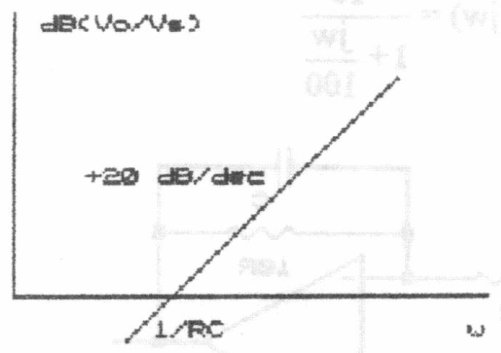
\includegraphics[width=0.4\linewidth]{_fig/op-amp_ejm1a_bode-derivador.png}
		\label{fig:op-amp_ejm1a_bode-derivador}
	}
	\caption{Diagrama de Bode (magnitud) de $Vo/Vs(jw)$}
	\label{fig:op-amp_ejm1a_bode}
\end{figure}

\textbf{Señal de entrada senoidal.} Si la señal de entrada a los circuitos de la figura \ref{fig:op-amp_ejm1} es sinusoidal, la función de transferencia será:

\begin{equation}
	\frac{Vo}{Vs}(jw) = - \frac{1}{jwRC} \quad \text{para el circuito integrador}
\end{equation}

\begin{equation}
	\frac{Vo}{Vs}(jw) = - jwRC \quad \text{para el circuito derivador}
\end{equation}

Una forma cómoda de visualizar la forma en que varía la magnitud y fase de $Vo/Vs$ con la frecuencia es a través del diagrama de Bode, descrito en el Anexo 2. El diagrama de Bode de magnitud de $Vo/Vs(jw)$ es un gráfico de $\text{dB} = 20\log|Vo/Vs(jw)|$ y se muestra para ambos circuitos en la figura 1.11.

\textbf{Ejemplo.} En el circuito de la figura \ref{fig:op-amp_ejm2_sch}, el amplificador operacional es ideal. $R = 1\text{ K}$; $C = 1\text{ uF}$. a) Dibujar el diagrama de magnitud de $Vo/Vs(jw)$. b) cuál es la magnitud de $Vo/Vs(jw = j200)$?

El circuito es un amplificador inversor con una función de transferencia:

\begin{equation}
	\frac{Vo}{Vs}(jw) = - \frac{Z_2}{Z_1} \quad \text{donde } Z_1 = R; \; Z_2 = 10R \,||\, \frac{1}{jwC}
\end{equation}

\begin{equation}
	\frac{Vo}{Vs}(jw) = - \frac{1}{1\text{K}} * \frac{10\text{K}}{1 + jw(10\text{K} * 1*10^{-6})}
\end{equation}

\begin{equation}
	\frac{Vo}{Vs}(jw) = \frac{-10}{1 + \frac{jw}{100}}
\end{equation}

\begin{figure}[h]
	\centering
	\subfloat[Circuito]
	{
		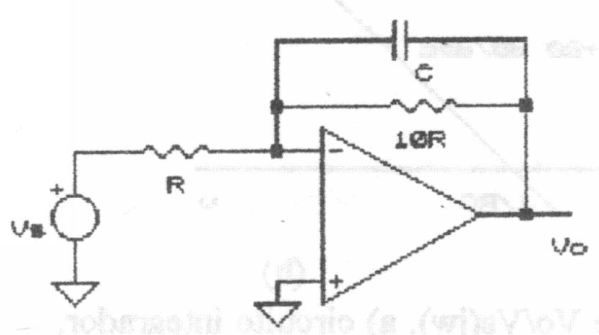
\includegraphics[width=0.4\linewidth]{_fig/op-amp_ejm2_sch.png}
		\label{fig:op-amp_ejm2_sch}
	}
	\subfloat[Diagrama de magnitud de $Vo/Vs(jw)$]
	{
		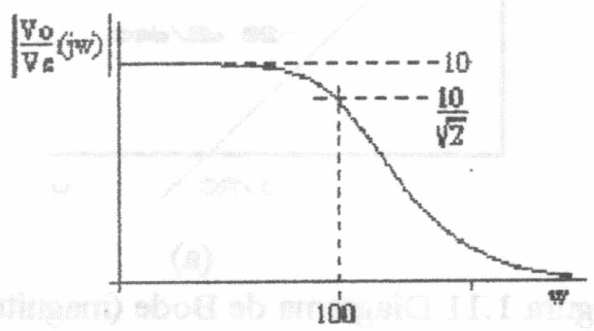
\includegraphics[width=0.4\linewidth]{_fig/op-amp_ejm2_bode.png}
		\label{fig:op-amp_ejm2_bode}
	}
	\caption{Ejemplo}
	\label{fig:op-amp_ejm2}
\end{figure}

\textbf{a)} El diagrama de magnitud de $(Vo/Vs)$ se muestra en la figura \ref{fig:op-amp_ejm2_bode}. El circuito se comporta como un circuito pasobajos. Se considera que el rango útil de amplificación incluye desde DC hasta aquella frecuencia $fo$ a la cual la ganancia cae a $1/\sqrt{2}$ de su máximo valor, en este caso, $10$. La frecuencia fo se llama frecuencia de corte del amplificador.

\textbf{b)} En $w = 200$, la magnitud de $Vo/Vs$ es:

\begin{equation}
	\left|\frac{Vo}{Vs}(j200)\right| = \frac{10}{\sqrt{1^2 + (200/100)^2}} = \frac{10}{\sqrt{5}} = 4.47
\end{equation}

\subsubsection{Circuito sumador}
Este circuito permite combinar linealmente varias señales:

La corriente en $R$ es la suma de las corrientes en las ramas de entrada. Esto es:

\begin{equation}
	I = I_1 + I_2 + ... + I_j + ....
\end{equation}

La tensión de salida $Vo$ está dada por:

\begin{equation}
	Vo = - I * R = - R * \left(\frac{V_1}{R_1} + \frac{V_2}{R_2} + ......\right)
\end{equation}

Si $R_1 = R_2 = R_3 = ... = R_n = R$:

\begin{equation}
	Vo = - (V_1 + V_2 + V_3 + ....)
\end{equation}

En estas condiciones, la señal de salida es proporcional a la suma de las señales de entrada.

\begin{figure}[h]
	\centering
	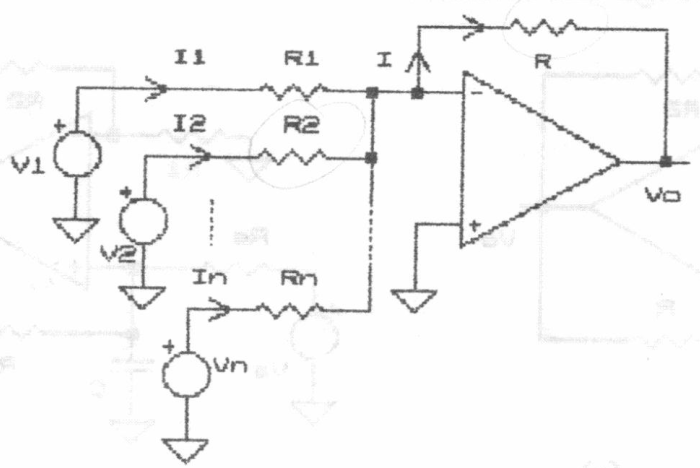
\includegraphics[width=0.6\linewidth]{_fig/op-amp_sumador.png}
	\caption{Circuito sumador}
	\label{fig:op-amp_sumador}
\end{figure}

La diferencia de potencial entre la entrada inversora y tierra es, en este caso, $0 volt$. Esto es, en este circuito existe una tierra virtual en la entrada inversora y no se producirá interacción entre las ramas de entrada.

\subsubsection{Convertidor de impedancia negativa}

El circuito de la figura \ref{fig:op-amp_conv-imp-neg-a} presenta una impedancia de entrada negativa a la fuente de señal $Vs$. En efecto:

\begin{figure}[h]
	\centering
	\subfloat[Circuito base]
	{
		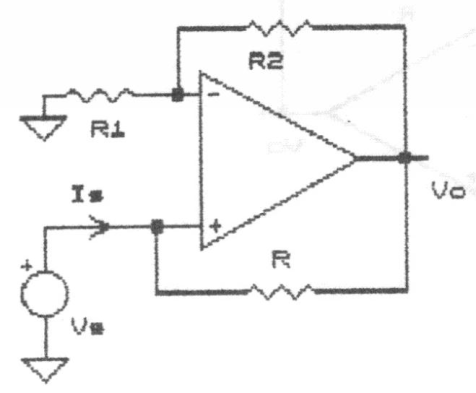
\includegraphics[width=0.4\linewidth]{_fig/op-amp_conv-imp-neg-a.png}
		\label{fig:op-amp_conv-imp-neg-a}
	}
	\subfloat[Integrador no inversor]
	{
		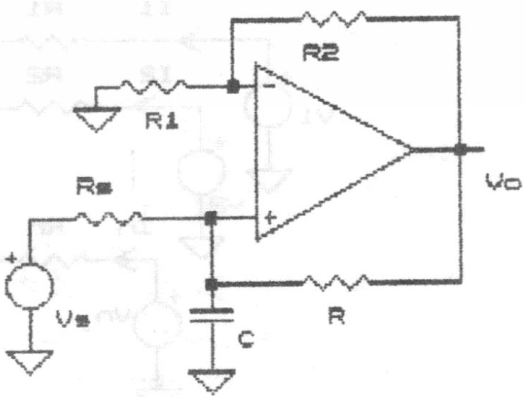
\includegraphics[width=0.4\linewidth]{_fig/op-amp_conv-imp-neg-b.png}
		\label{fig:op-amp_conv-imp-neg-b}
	}
	\caption{Convertidor de impedancia negativa}
	\label{fig:op-amp_conv-imp-neg}
\end{figure}

\begin{equation}
	Is = \frac{Vs - Vo}{R}
\end{equation}

La tensión $Vo$ corresponde a la señal de salida de un amplificador no inversor con una señal de entrada $V^+ = Vs$. Por lo tanto:

\begin{equation}
	Vo = \left(1 + \frac{R_2}{R_1}\right) * Vs
\end{equation}

Así:

\begin{equation}
	Is = - \frac{R_2}{R_1} * \frac{Vs}{R}
\end{equation}

\begin{equation}
	Zi = \frac{Vs}{Is} = - \frac{R_1}{R_2} * R
\end{equation}

Esto es, el circuito entrega una corriente a la fuente $Vs$.

\textbf{Ejemplo.} En la figura \ref{fig:op-amp_conv-imp-neg-b} se muestra un integrador no inversor implementado con un convertidor de impedancia negativa. Comprobar que, si $R_1 = R_2$ y $Rs = R$, la tensión de salida estará dada por:

\begin{equation}
	Vo = \frac{1}{RC} \int Vs \, dt
\end{equation}

\section{Amplificador operacional real}
En aplicaciones en que se requiera una mayor precisión, es necesario considerar otros efectos, de diverso origen, que afectan desfavorablemente la respuesta del amplificador operacional. Entre estos efectos mencionaremos, por ahora, los siguientes:

\begin{itemize}
	\item ganancia finita y dependiente de la frecuencia.
	\item impedancia de entrada finita.
	\item impedancia de salida diferente de cero.
	\item tensión de desbalance (offset) de la entrada.
	\item corriente de polarización y de desbalance en las entradas.
	\item corriente limitada en el terminal de salida.
\end{itemize}

Aún cuando en la práctica éstas y otras imperfecciones se presentan en forma simultánea, se consideran separadamente para facilitar el análisis de su efecto en un circuito.

\subsection{Ganancia finita y dependiente de la frecuencia}
La ganancia de los amplificadores operacionales reales más comúnmente usados (amplificadores compensados) es finita y dependiente de la frecuencia:

\begin{equation}
	Av = \frac{Avo}{1 + jf/f_H}
\end{equation}

En esta relación, $A_vo$ es un número real y positivo que representa la ganancia diferencial del amplificador a baja frecuencia ($f \ll f_H$). $f_H$ es la llamada frecuencia de corte del amplificador operacional. El módulo de la ganancia del amplificador operacional disminuye al aumentar la frecuencia, desde $A_vo$ ($f=0$) hacia $0$ ($f \to \infty$). En la frecuencia de corte ($fc = f_H$), el módulo de la ganancia $A_v$ del amplificador operacional ha caído a $Avo / \sqrt{2}$. A frecuencias muy bajas la fase de Av es cercana a $0^\circ$ y se acerca a $-90^\circ$ a frecuencias muy elevadas respecto a $f_H$.

\subsubsection{Ancho de banda}
El ancho de banda (BW) de un amplificador es el rango de frecuencias en el cual el módulo de la ganancia tiene una magnitud mayor o igual que $1/\sqrt{2}$ veces su máximo valor. En el caso del amplificador operacional, este máximo valor es $A_vo$ y el ancho de banda cubre la región comprendida entre $f = 0$ ($DC$) y la frecuencia de corte $f_H$. Esto es, el ancho de banda del amplificador operacional es $\text{BW} = f_H - 0 = f_H$.

\begin{figure}[h]
	\centering
	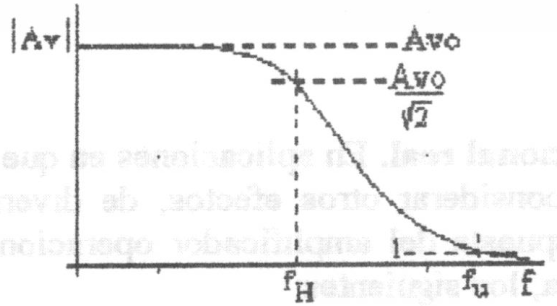
\includegraphics[width=0.6\linewidth]{_fig/op-amp_ancho-banda_av.png}
	\caption{Diagrama de magnitud de de $A_v$}
	\label{fig:op-amp_ancho-banda_av}
\end{figure}

Se define producto ganancia-ancho de banda (PGAB) o frecuencia de ganancia unitaria ($f_u$) del amplificador operacional a:

\begin{equation}
	\text{PGAB} = f_u = \text{Avo} * f_H
\end{equation}

En un amplificador tipo uA741 el valor típico de PGAB es de $1.5\text{ MHz}$. La ganancia $Vo/Vs$ y la impedancia de entrada $Zi$ de un amplificador se verán afectadas por esta variación de Av con la frecuencia. A modo de ejemplo, se había encontrado la siguiente expresión para la ganancia en el amplificador inversor de la figura \ref{fig:op-amp_inversor}, repetida por comodidad en la figura \ref{fig:op-amp_ancho-banda_av}:

\begin{equation}
	\frac{Vo}{Vs} = \frac{- Av}{1 + (1 + Av) * \frac{R_1}{R_2}}
\end{equation}

Reemplazando en esta expresión $Av = A_{vo} / (1 + jf/f_H)$ y después de alguna manipulación algebraica esta expresión puede ser escrita como:

\begin{equation}
	\frac{Vo}{Vs} = \frac{Ko}{1 + jf/f_o}
\end{equation}

\begin{equation}
	Ko = \frac{-(R_2/R_1) * A_{vo}}{A_{Ao} + 1 + R_2/R_1}
\end{equation}

$Ko$: ganancia a baja frecuencia del amplificador inversor

\begin{equation}
	f_o = \frac{f_H * (1 + R_2/R_1 + A_{vo})}{1 + R_2/R_1}
\end{equation}

$f_o$: frecuencia de corte del amplificador inversor, esto es, frecuencia a la cual la ganancia cae a $1/\sqrt{2}$ de su valor a baja frecuencia ($Ko$). Esto es equivalente a decir que en el diagrama de magnitud, $20 \log|Vo/Vs|$ cae $3\text{ dB}$ respecto de su valor a baja frecuencia.

Si $A_{vo} \gg R_2/R_1 \gg 1$, las expresiones para $K_o$ y $f_c$ se reducen a:

\begin{equation}
	|Ko| = \frac{R_2}{R_1}
\end{equation}

\begin{equation}
	f_o = \frac{f_H * \text{Avo}}{R_2/R_1}
\end{equation}

\begin{equation}
	|Ko| * f_o = \text{Avo} * f_H = f_T
\end{equation}

En esta última expresión se observa que, en las condiciones señaladas, el producto ganancia-ancho de banda $f_T$ del amplificador inversor es aproximadamente igual al producto ganancia-ancho de banda del amplificador operacional. En aplicaciones prácticas, el mínimo valor especificado por el fabricante para el producto ganancia-ancho de banda del amplificador operacional que se desea usar debe ser mayor que el producto ganancia-ancho de banda requerido por la aplicación. En un amplificador no inversor puede obtenerse una expresión similar para el producto ganancia-ancho de banda.

\begin{figure}[h]
	\centering
	\subfloat[Amplificador inversor]
	{
		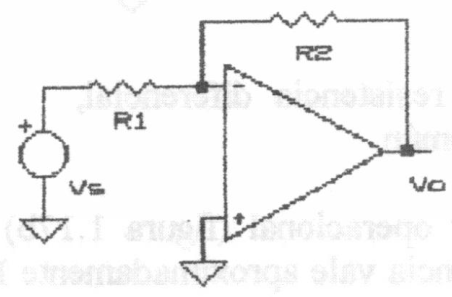
\includegraphics[width=0.4\linewidth]{_fig/op-amp_ancho-banda_inv_sch.png}
		\label{fig:op-amp_ancho-banda_inv_sch}
	}
	\subfloat[diagrama de magnitud de $Vo/Vs$]
	{
		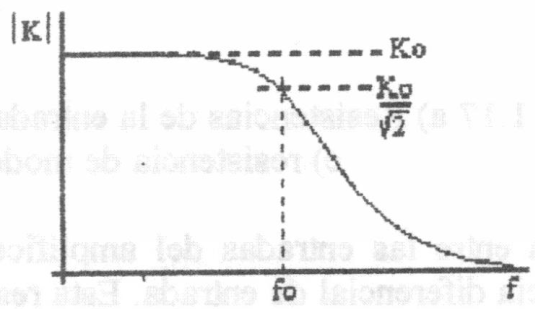
\includegraphics[width=0.4\linewidth]{_fig/op-amp_ancho-banda_inv_bode.png}
		\label{fig:op-amp_ancho-banda_inv_bode}
	}
	\caption{Convertidor de impedancia negativa}
	\label{fig:op-amp_ancho-banda_inv}
\end{figure}

\textbf{Ejemplo.} Si en el amplificador inversor anterior se requiere una ganancia con un valor $|Ko| = 20$, determinar la frecuencia de corte alta típica que puede obtenerse de los siguientes amplificadores operacionales: a) uA741, b) LF357, c) AD5539. La frecuencia de corte alta del amplificador inversor está dada en forma aproximada por: $f_o = \text{Avo} * f_H / |Ko|$. El valor típico del producto ganancia-ancho de banda de los amplificadores operacionales y la frecuencia típica de corte alta que se obtendría en esta aplicación se tabulan a continuación:

\begin{center}
	\begin{tabular}{ccc}
		\textbf{Amplificador} & \textbf{PGAB = Avo * $\mathbf{f_H}$ (MHz)} & \textbf{$\mathbf{f_o}$ = PGAB/|Ko| (KHz)} \\
		uA741 & 1.5 & 75 \\
		LF357 & 20 & 1000 \\
		AD5539 & 1400 & 70000
	\end{tabular}
\end{center}

Se observa que en un amplificador implementado con estos amplificadores operacionales, la frecuencia de corte alta es muy superior si se usa un AD5539.

\subsection{Resistencia de entrada finitas}
El circuito equivalente simplificado, presentado en la figura \ref{fig:op-amp_ejm2_sch}, tiene ambas entradas aisladas del resto del circuito. Sin embargo, el circuito equivalente de la figura \ref{fig:op-amp_ref_rin} representa más acertadamente el comportamiento de las entradas de un amplificador operacional real.

\begin{figure}[h]
	\centering
	\subfloat[Resistencias de la entrada]
	{
		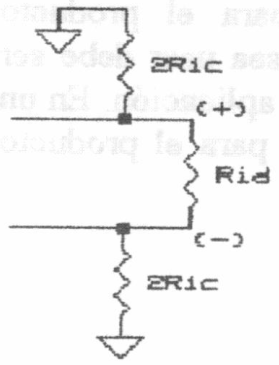
\includegraphics[width=0.25\linewidth]{_fig/op-amp_ref_rin.png}
		\label{fig:op-amp_ref_rin}
	}
	\subfloat[resistencia diferencial]
	{
		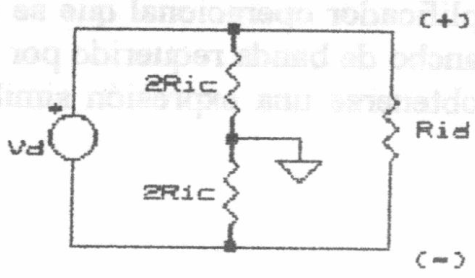
\includegraphics[width=0.35\linewidth]{_fig/op-amp_ref_rdiff.png}
		\label{fig:op-amp_ref_rdiff}
	}
	\subfloat[resistencia de modo común]
	{
		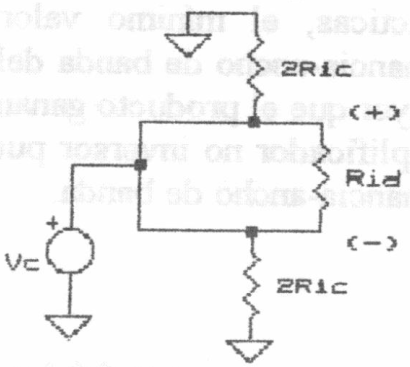
\includegraphics[width=0.3\linewidth]{_fig/op-amp_ref_rcomun.png}
		\label{fig:op-amp_ref_rcomun}
	}
	\caption{Resistencia de entrada finitas}
	\label{fig:op-amp_ref_r}
\end{figure}

La resistencia entre las entradas del amplificador operacional (figura \ref{fig:op-amp_ref_rdiff}) se llama resistencia diferencial de entrada. Esta resistencia vale aproximadamente $Rid$ pues, prácticamente, para todos los amplificadores operacionales reales se verifica que $Rid \ll Ric$. Por otra parte, si se verifica esta misma desigualdad, la resistencia entre las entradas y tierra (figura \ref{fig:op-amp_ref_rcomun}) es $Ric$.

\textbf{Ejemplo.} En el circuito inversor de la figura \ref{fig:op-amp_ref_inv-sch}, la tensión $Vi$ puede ser expresada mediante:

\begin{equation}
	Vi = \frac{Vs * \dfrac{G_1}{G_1 + G_2 + Gid}}{1 + Av * \dfrac{G_2}{G_1 + G_2 + Gid}}
\end{equation}

\begin{equation}
	Vo = Av * Vi; \quad G_1 = 1/R_1; \quad G_2 = 1/R_2; \quad Gid = 1/Rid
\end{equation}

\begin{figure}[h]
	\centering
	\subfloat[circuito]
	{
		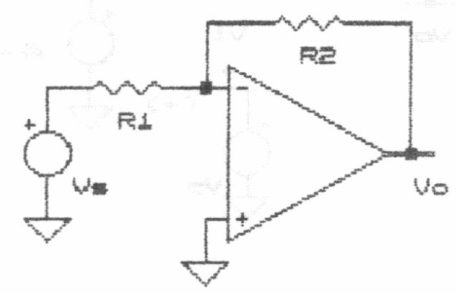
\includegraphics[width=0.4\linewidth]{_fig/op-amp_ref_inv-sch.png}
		\label{fig:op-amp_ref_inv-sch}
	}
	\subfloat[circuito equivalente considerando Rid y Ric finitos]
	{
		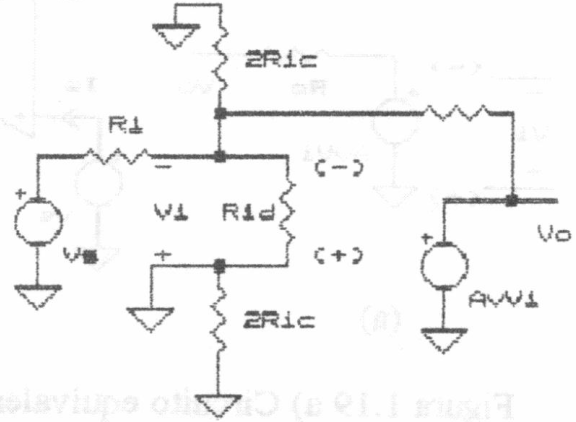
\includegraphics[width=0.4\linewidth]{_fig/op-amp_ref_inv-eq.png}
		\label{fig:op-amp_ref_inv-eq}
	}
	\caption{Amplificador inversor}
	\label{fig:op-amp_ref_inv}
\end{figure}

En estas últimas expresiones se observa que si $Av \to \infty$, la tensión $Vi \to 0$ y $Vo/Vs \to -R_2/R_1$. Esto es, si el amplificador operacional tiene una ganancia $Av$ infinita, las resistencias $Rid$ y $Ric$ no tendrán efecto sobre la ganancia, $K = Vo/Vs$, ni sobre la impedancia de entrada del circuito, $Zi = Vs/Is$. En general, el efecto de valores finitos de $Rid$ y $Ric$ en la ganancia e impedancia de entrada, es menos significativo que el efecto de una ganancia finita y dependiente de la frecuencia. En todo caso, en aplicaciones en que la fuente de señal tenga asociada una impedancia en serie elevada, se deberá recurrir al uso de amplificadores operacionales con entrada FET que tienen una impedancia de entrada muy elevada.

\subsection{Resistencia de salida}
En amplificadores operacionales reales existe una resistencia, Ro, en serie con la fuente dependiente $Av * Vi$, tal como se muestra en la figura \ref{fig:op-amp_ejm7}:

\textbf{Ejemplo.} En el seguidor de voltaje de la figura \ref{fig:op-amp_ejm7_a} se cumple:

\begin{equation}
	Is = 0; \quad Zi = \frac{Vs}{Is} = \infty
\end{equation}

\begin{equation}
	Vs - Vi = Av * Vi; \quad Vi = \frac{Vs}{1 + Av}; \quad Vo = \frac{Av * Vs}{1 + Av}
\end{equation}

\begin{figure}[h]
	\centering
	\subfloat[Circuito equivalente incluyendo Ro]
	{
		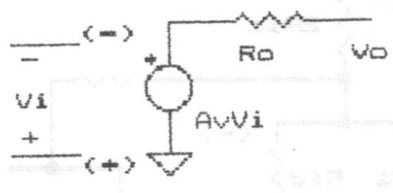
\includegraphics[width=0.3\linewidth]{_fig/op-amp_ejm7_a.png}
		\label{fig:op-amp_ejm7_a}
	}
	\subfloat[Seguidor de voltaje]
	{
		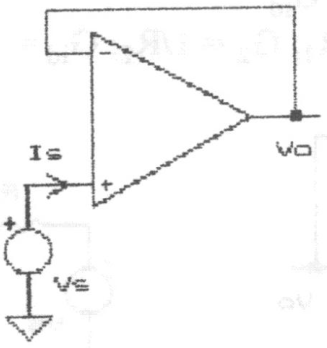
\includegraphics[width=0.3\linewidth]{_fig/op-amp_ejm7_b.png}
		\label{fig:op-amp_ejm7_b}
	}
	\subfloat[Circuito equivalente]
	{
		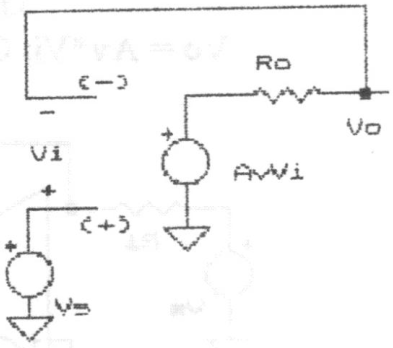
\includegraphics[width=0.3\linewidth]{_fig/op-amp_ejm7_c.png}
		\label{fig:op-amp_ejm7_c}
	}
	\caption{Resistencia de entrada finitas}
	\label{fig:op-amp_ejm7}
\end{figure}

Para un 741, ($\text{Avo} = 100000$), la ganancia del circuito es muy cercana a la unidad. En el circuito estudiado, la resistencia Ro no tiene mayor efecto sobre la impedancia de entrada ni la ganancia de tensión. El efecto de $\text{Ro} \neq 0$ se manifiesta principalmente sobre la impedancia de salida del circuito.

\textbf{Definición.} Impedancia de salida de un circuito es la impedancia equivalente (Thevenin) vista entre los bornes de salida del circuito. Para su determinación es necesario reemplazar las fuentes de tensión independientes por cortocircuitos y las fuentes de corriente independientes por circuitos abiertos.

\begin{figure}[h]
	\centering
	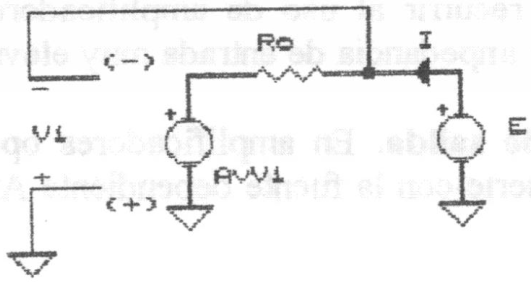
\includegraphics[width=0.6\linewidth]{_fig/op-amp_ejm7_zo.png}
	\caption{Determinación de la impedancia de salida}
	\label{fig:op-amp_ejm7_zo}
\end{figure}

En el circuito anterior (ver figura \ref{fig:op-amp_ejm7_zo}):

\begin{equation}
	I = \frac{E - Av * Vi}{Ro}; \quad Vi = -E
\end{equation}

\begin{equation}
	I = \frac{E(1 + Av)}{Ro}; \quad Zo = \frac{E}{I} = \frac{Ro}{1 + Av}
\end{equation}

En un amplificador uA741, $\text{Avo} = 5 * 10^4$, $f_H = 8\text{ Hz}$, $\text{Ro} = 75\text{ ohm}$[cite: 23]. Así, en baja frecuencia, $Zo = 75 / (1 + 5 * 10^4) = 1.5 * 10^{-3}\text{ ohm}$. Para una frecuencia de $100\text{ KHz}$, $Av = -j4$ y la impedancia de salida vale ahora $Zo = 75 / (1 - j4)$, esto es, la magnitud de Zo ha aumentado a $18.19\text{ ohm}$.

En otras configuraciones amplificadoras, la impedancia de salida puede calcularse usando un procedimiento similar.

\subsection{Corrientes de polarización en las entradas}

Es necesario suministrar corrientes dc a las entradas de un amplificador operacional real para que éste opere satisfactoriamente. Ver figura \ref{fig:op-amp_cpe}.

\begin{figure}[h]
	\centering
	\subfloat[Simbolo]
	{
		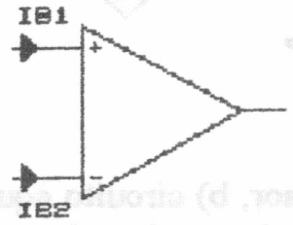
\includegraphics[width=0.4\linewidth]{_fig/op-amp_cpe_simbolo.png}
		\label{fig:op-amp_cpe_simbolo}
	}
	\subfloat[Equivalente]
	{
		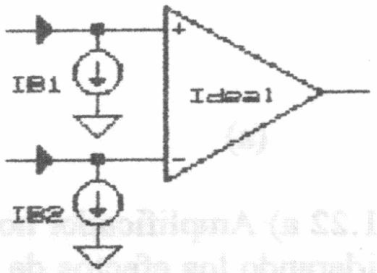
\includegraphics[width=0.4\linewidth]{_fig/op-amp_cpe_eq.png}
		\label{fig:op-amp_cpe_eq}
	}
	\caption{Modelo del amplificador operacional que considera las corrientes de polarización en las entradas}
	\label{fig:op-amp_cpe}
\end{figure}

El modelo incluye un amplificador operacional ideal y dos fuentes de corriente continua, $I_{B1}$ e $I_{B2}$. Para un amplificador operacional dado, la magnitud de estas corrientes, $I_{B1}$ e $I_{B2}$, depende de la polarización, la temperatura y es independiente de la magnitud de la señal aplicada. De acuerdo a la convención de cuadripolos (la corriente que entra a un terminal activo es positiva), estas corrientes pueden ser ambas positivas o ambas negativas. Se define:

\begin{equation}
	I_B = \frac{I_{B1} + I_{B2}}{2}, \quad \text{corriente de polarización}
\end{equation}

\begin{equation}
	I_{OS} = I_{B1} - I_{B2}, \quad \text{corriente de desbalance de las entradas}
\end{equation}

Así, las corrientes $I_{B1}$ e $I_{B2}$ pueden ser expresadas:

\begin{equation}
	I_{B1} = I_B + \frac{I_{OS}}{2}
\end{equation}

\begin{equation}
	I_{B2} = I_B - \frac{I_{OS}}{2}
\end{equation}

El signo de $I_B$ depende de la estructura interna del amplificador operacional. Por su parte, $I_{OS}$ puede ser positivo o negativo. La polaridad de $I_{OS}$ puede cambiar al cambiar la tensión de polarización o la temperatura de operación.

\begin{figure}[h]
	\centering
	\subfloat[Circuito]
	{
		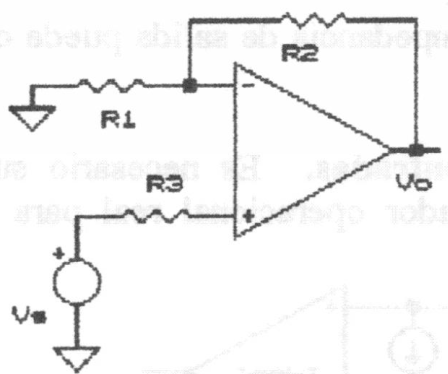
\includegraphics[width=0.4\linewidth]{_fig/op-amp_cpe_n-inv_sch.png}
		\label{fig:op-amp_cpe_n-inv_sch}
	}
	\subfloat[Equivalente considerando los efectos de las corrientes de polarización]
	{
		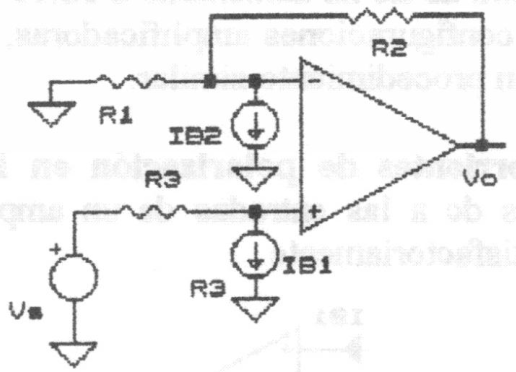
\includegraphics[width=0.4\linewidth]{_fig/op-amp_cpe_n-inv_eq.png}
		\label{fig:op-amp_cpe_n-inv_eq}
	}
	\caption{Amplificador no inversor}
	\label{fig:op-amp_cpe_inv-cei}
\end{figure}

\textbf{Ejemplo.} Encontrar una expresión para la tensión de salida del circuito no inversor de la figura \ref{fig:op-amp_cpe_inv-cei} considerando las corrientes de polarización en las entradas del amplificador operacional.

Al aplicar superposición al circuito anterior se obtiene:

\textbf{a) $Vs \neq 0$; $I_{B1} = 0$; $I_{B2} = 0$}

\begin{equation}
	Vo' = \left(1 + \frac{R_2}{R_1}\right) * Vs
\end{equation}

\textbf{b) $Vs = 0$; $I_{B1} \neq 0$; $I_{B2} = 0$}

\begin{equation}
	Vo'' = -I_{B1} * R_3 * \left(1 + \frac{R_2}{R_1}\right) = - \left(I_B + \frac{I_{OS}}{2}\right) * R_3 * \left(1 + \frac{R_2}{R_1}\right)
\end{equation}

\textbf{c) $Vs = 0$; $I_{B1} = 0$; $I_{B2} \neq 0$}

\begin{equation}
	Vo''' = I_{B2} * R_2 = \left(I_B - \frac{I_{OS}}{2}\right) * R_2
\end{equation}

\noindent La señal de salida total será:

\begin{equation}
	Vo = Vs * \left(1 + \frac{R_2}{R_1}\right) + I_B * \left[R_2 - R_3 \left(1 + \frac{R_2}{R_1}\right)\right] - \frac{I_{OS}}{2} \left[R_2 + R_3 \left(1 + \frac{R_2}{R_1}\right)\right]
\end{equation}

\noindent Se observa que el término con $I_B$ se anula si $R_3 = R_1 \,||\, R_2$. En este caso:

\begin{equation}
	Vo = Vs * \left(1 + \frac{R_2}{R_1}\right) - I_{OS} * R_2
\end{equation}

\subsubsection{Influencia de la temperatura}
La magnitud de las corrientes de polarización en las entradas depende de la temperatura y la tensión de polarización. Los fabricantes publican curvas y tablas que muestran la forma en que varían $I_B$ e $I_{OS}$ en un rango de temperaturas dado y para una cierta tensión de polarización o, alternativamente, incluye en la hoja de datos el máximo valor que pueden tomar estas corrientes en el rango normal de temperaturas de operación del amplificador operacional.

Generalmente, el efecto de las corrientes de polarización puede ser ignorado en aplicaciones simples. En aplicaciones de precisión, el efecto de estas corrientes puede ser llevado a niveles insignificantes utilizando amplificadores operacionales de baja corriente de polarización. Es posible conseguir amplificadores operacionales con corrientes de polarización, $I_B$, por debajo de $1\text{ pA}$ (año 1991).

\textbf{Ejemplo.} En el circuito amplificador no inversor de la figura 1.22, $R_1 = 10\text{ K}$, $R_2 = 470\text{ K}$ y $R_3 = R_1 \,||\, R_2$, determinar la contribución a la tensión de salida de las corrientes de polarización si la temperatura varía entre $25$ y $100^\circ\text{ C}$ y se usa un amplificador operacional tipo a) uA741; b) OPA111.

Si $R_3 = R_1 \,||\, R_2$, la contribución de las corrientes de polarización a la tensión de salida consistirá únicamente en el término $-I_{OS} * R_2$. Este término produce un error en $Vo$ cuya magnitud depende de la temperatura y que puede ser muy importante en aplicaciones en las que el circuito maneje señales de pequeña magnitud que varíen lentamente.

\textbf{a)} Para un amplificador uA741, en el rango de temperatura de operación, la corriente $I_{OS}$ tiene un valor máximo de $200\text{ nA}$. Así, la tensión de salida tendrá una componente debida a $I_{OS}$ con una magnitud máxima de $200 * 10^{-9} * 470 * 10^3 = 0.094\text{ volt}$.

\textbf{b)} En el amplificador OPA111, el valor máximo de la corriente de desbalance, $I_{OS}$ es de $3.1\text{ nA}$. Así:

\begin{equation}
	I_{OS} * R_2 = 3.1\text{ nA} * 470 * 10^3 = 1.5\text{ mV}
\end{equation}

Se observa que el error máximo, producido en la tensión de salida, es substancialmente menor en el caso del amplificador tipo OPA111. En aplicaciones que requieran una precisión elevada se deberá elegir el amplificador operacional considerando, entre otros parámetros, los valores de $I_B$ e $I_{OS}$.

La estructura de un circuito práctico debe contemplar la necesidad de permitir libremente la circulación hacia tierra de las corrientes de polarización. En la figura \ref{fig:op-amp_it} se muestran circuitos que no funcionarán correctamente por no satisfacer este requisito.

\begin{figure}[h]
	\centering
	\subfloat[A]
	{
		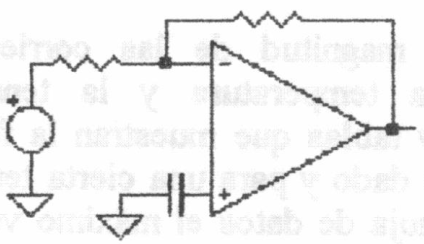
\includegraphics[width=0.4\linewidth]{_fig/op-amp_it_a.png}
		\label{fig:op-amp_it_a}
	}
	\subfloat[B]
	{
		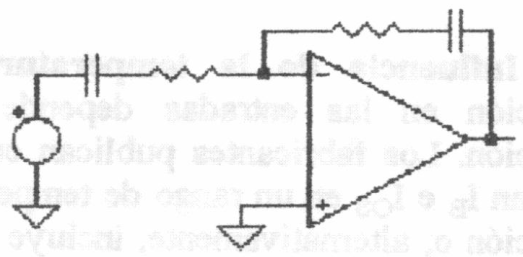
\includegraphics[width=0.4\linewidth]{_fig/op-amp_it_b.png}
		\label{fig:op-amp_it_b}
	}
	\caption{Circuitos que funcionan pues no permiten la circulación de las corrientes de polarización}
	\label{fig:op-amp_it}
\end{figure}

\subsection{Tensión de desbalance de las entradas, $V_{OS}$}
Idealmente, un amplificador operacional amplifica la diferencia entre las señales aplicadas a sus entradas.

\begin{equation}
	Vo = Av * (V^+ - V^-)
\end{equation}

\begin{figure}[h]
	\centering
	\subfloat[$V^+ = V^-$, $Vo \neq 0$]
	{
		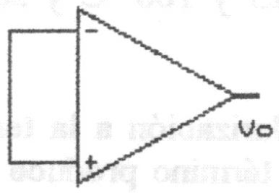
\includegraphics[width=0.3\linewidth]{_fig/op-amp_tde-vos_a.png}
		\label{fig:op-amp_tde-vos_a}
	}
	\subfloat[$V^+ = V^- + V_{OS}$, $Vo = 0$]
	{
		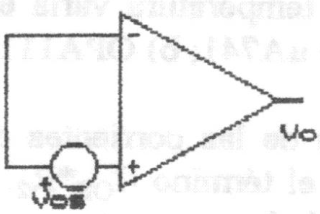
\includegraphics[width=0.3\linewidth]{_fig/op-amp_tde-vos_b.png}
		\label{fig:op-amp_tde-vos_b}
	}
	\subfloat[Modelo para la tensión de desbalance]
	{
		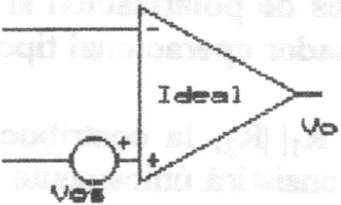
\includegraphics[width=0.3\linewidth]{_fig/op-amp_tde-vos_c.png}
		\label{fig:op-amp_tde-vos_c}
	}
	\caption{Tensión de desbalance de entradas, $V_{OS}$}
	\label{fig:op-amp_tde-vos}
\end{figure}

Si se cortocircuita las entradas, como se muestra en la figura \ref{fig:op-amp_tde-vos_a}, la tensión de salida debería ser cero pues $V^+ = V^-$. Sin embargo, al realizar este experimento en un amplificador operacional real se observa que la tensión de salida es diferente de cero. Es necesario aplicar una pequeña tensión $V_{OS}$ en serie con las entradas, como se muestra en la figura \ref{fig:op-amp_tde-vos_b}, para llevar la tensión de salida a cero.

\noindent El modelo del amplificador operacional real incluye un amplificador operacional ideal que tiene una fuente de tensión $V_{OS}$ en serie con su entrada inversora. La magnitud y polaridad de $V_{OS}$ varían, al igual que las corrientes de polarización, con la temperatura. El fabricante publica en la hoja de datos el valor de $V_{OS}$ a $25^\circ\text{ C}$ y $d(V_{OS})/dT$. Si la temperatura de operación es $\text{Ta} \neq 25^\circ\text{ C}$, el valor de $V_{OS}(\text{Ta})$ puede ser encontrado usando:

\begin{equation}
	V_{OS}(\text{Ta}) = V_{OS}(25^\circ\text{ C}) + (\text{Ta} - 25^\circ\text{ C}) * \frac{dV_{OS}}{dT}
\end{equation}

\textbf{Ejemplo.} Hallar la tensión de salida total en el amplificador inversor de la figura \ref{fig:op-amp_ejm-tde-vos}. 

El circuito opera en un rango de temperatura que varía entre $25$ y $70^\circ\text{ C}$ e incluye un amplificador operacional tipo uA777 con $V_{OS}(\text{máx}) = 5\text{ mV}$ y $d(V_{OS})/dt(\text{máx}) = 30\text{ uV}/^\circ\text{ C}$. El efecto de $I_B$ e $I_{OS}$ puede ser ignorado.

\begin{figure}[h]
	\centering
	\subfloat[Amplificador inversor]
	{
		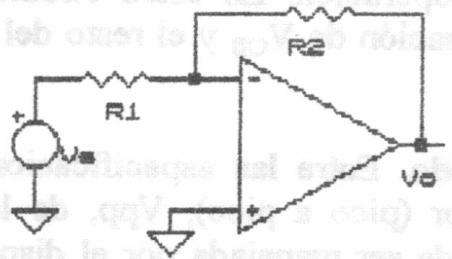
\includegraphics[width=0.4\linewidth]{_fig/op-amp_ejm-tde-novos_sch.png}
		\label{fig:op-amp_ejm-tde-novos_sch}
	}
	\subfloat[circuito equivalente incluyendo $V_{OS}$]
	{
		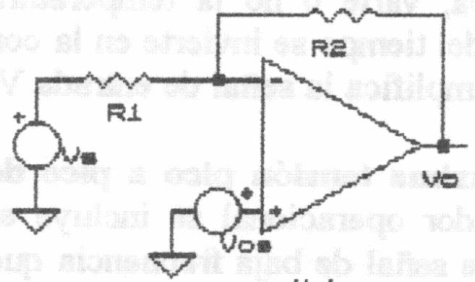
\includegraphics[width=0.4\linewidth]{_fig/op-amp_ejm-tde-vos_sch.png}
		\label{fig:op-amp_ejm-tde-vos_sch}
	}
	\caption{Tensión de desbalance de las entradas, $V_{OS}$}
	\label{fig:op-amp_ejm-tde-vos}
\end{figure}

La tensión de salida será:

\begin{equation}
	Vo = - \frac{R_2}{R_1} * Vs + \left(1 + \frac{R_2}{R_1}\right) * V_{OS}
\end{equation}

En estas condiciones, la máxima tensión de desbalance en la entrada variará entre $V_{OS}(25^\circ\text{ C}) = 5\text{ mV}$ y $V_{OS}(70^\circ\text{ C}) = 5\text{ mV} + (70 - 25) * 30\text{ uV}$, esto es, $6.35\text{ mV}$. En el circuito, $R_2/R_1 = 100$. La señal de salida tendrá una componente debida a $V_{OS}$ con una magnitud que variará entre $0.505$ y $0.641\text{ volt}$.

\begin{figure}[h]
	\centering
	\subfloat[terminales especiales]
	{
		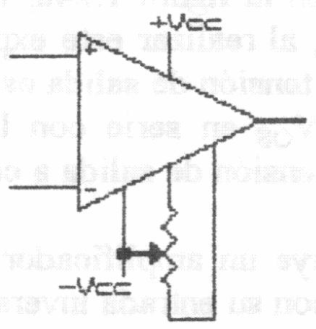
\includegraphics[width=0.4\linewidth]{_fig/op-amp_ejm-tde-novos_comp-a.png}
		\label{fig:op-amp_ejm-tde-novos_comp-a}
	}
	\subfloat[agregando una tensión dc en serie]
	{
		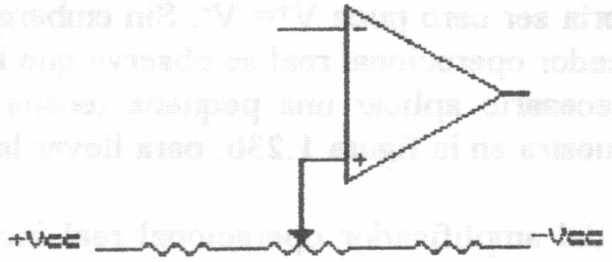
\includegraphics[width=0.4\linewidth]{_fig/op-amp_ejm-tde-novos_comp-b.png}
		\label{fig:op-amp_ejm-tde-novos_comp-b}
	}
	\caption{Compensación de $V_{OS}$}
	\label{fig:op-amp_ejm-tde-novos_comp}
\end{figure}

\subsubsection{Compensación de la tensión $V_{OA}$}
Algunos amplificadores cuentan con terminales para la conexión de redes externas que permiten compensar la tensión de desbalance. En amplificadores operacionales que no dispongan de este tipo de terminales se puede agregar tensiones dc en serie para compensar el efecto de $V_{OS}$ a una cierta temperatura. En el ejemplo anterior, si se efectúa el ajuste de la red de compensación a $25^\circ\text{ C}$, la magnitud de la componente de Vo debida a $V_{OS}$ variará entre $0\text{ volt}$ ($25^\circ\text{ C}$) y $0.136\text{ volt}$ ($70^\circ\text{ C}$).

En aplicaciones de alta precisión, se usan amplificadores operacionales tipo chopper en los que se efectúa periódicamente la compensación de $V_{OS}$, en forma automática, varíe o no la temperatura de operación. En estos circuitos, cierta fracción del tiempo se invierte en la compensación de $V_{OS}$ y el resto del tiempo el circuito amplifica la señal de entrada $Vs$.

\subsection{Máxima tensión pico a pico de salida}
Entre las especificaciones de un amplificador operacional se incluye el valor (pico a pico), Vpp, de la máxima tensión de señal de baja frecuencia que puede ser manejada por el dispositivo en ciertas condiciones de polarización (valor de $\pm\text{ Vcc}$). Vpp depende de la estructura interna del amplificador operacional y se acerca apreciablemente a $2*\text{ Vcc}$ en amplificadores operacionales tipo MOS.

\begin{figure}[h]
	\centering
	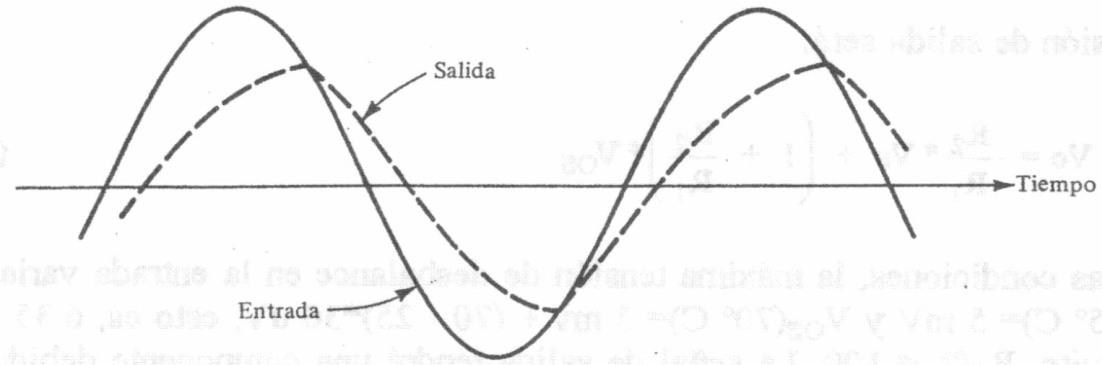
\includegraphics[width=0.6\linewidth]{_fig/op-amp_mtpps.png}
	\caption{Deformación de la señal de salida ($f > f_M$)}
	\label{fig:op-amp_mtpps}
\end{figure}

\subsection{Frecuencia de plena potencia fin y Slew Rate}
La especificación de máxima tensión de salida es válida sólo si la frecuencia de la señal está por debajo de un cierto valor llamado frecuencia de plena potencia, $f_M$. Si se aumenta la frecuencia por encima de $f_M$ se reduce la amplitud de la señal de salida y, además, se produce una deformación de ésta, tal como se muestra en la figura \ref{fig:op-amp_mtpps}. Esto se debe a que la velocidad de cambio de la tensión de salida no puede exceder un cierto valor límite llamado Slew Rate, SR, expresado en volt/seg.

La especificación de Slew Rate se establece en un circuito seguidor de voltaje (figura \ref{fig:op-amp_sr}) excitado por una señal de entrada cuadrada. La señal de salida tiene la forma mostrada en la figura anterior y el módulo de la pendiente en las transiciones corresponde al valor de SR.

\begin{figure}[h]
	\centering
	\subfloat[terminales especiales]
	{
		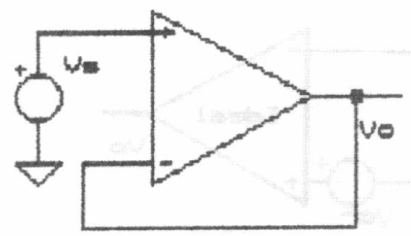
\includegraphics[width=0.4\linewidth]{_fig/op-amp_sr_sch.png}
		\label{fig:op-amp_sr_sch}
	}
	\subfloat[agregando una tensión dc en serie]
	{
		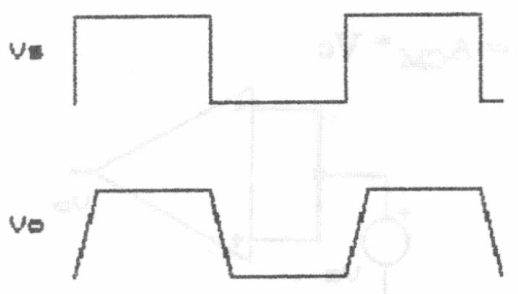
\includegraphics[width=0.4\linewidth]{_fig/op-amp_sr_vsvo.png}
		\label{fig:op-amp_sr_vsvo}
	}
	\caption{Determinación de SR}
	\label{fig:op-amp_sr}
\end{figure}

La frecuencia de plena potencia, $f_M$, puede ser relacionada con el valor de SR: una señal de salida sinusoidal con la máxima amplitud de salida que puede manejar el amplificador ($\text{Vpp}/2$), sin producir distorsión, puede ser expresada mediante:

\begin{equation}
	Vo = \frac{Vpp}{2} \text{ sen}(wt) = \frac{Vpp}{2} \text{ sen}(2\pi f t)
\end{equation}

La máxima pendiente de esta onda sinusoidal a la frecuencia $f_M$ corresponde al valor de SR. Esto es:

\begin{equation}
	\left|\frac{dVo}{dt}\right|_{\text{MAX}} = \frac{Vpp}{2} * 2\pi f_M = \text{SR}
\end{equation}

\begin{equation}
	f_M = \frac{\text{SR}}{2\pi * (\text{Vpp}/2)}
\end{equation}

\textbf{Ejemplo.} En un amplificador operacional tipo 741 el valor de SR especificado por el fabricante es $0.5\text{ volt/us}$. Si la señal de salida tiene una amplitud de $5\text{ volt}$ ($10\text{ volt}$ pico a pico), la máxima frecuencia de una señal senoidal que no experimentará deformación por efecto de SR es de $15900\text{ Hz}$.

\subsection{Razón de rechazo de modo común}
Idealmente, la señal de salida de un amplificador operacional depende únicamente de la señal diferencial de entrada $Vi = V^+ - V^-$. En un amplificador operacional real, la señal de salida depende también del valor promedio $Vc$ del las tensiones presentes en ambas entradas llamado también señal de modo común.

En el circuito de la figura \ref{fig:op-amp_rrmc-a}, la señal de salida es:

\begin{equation}
	Vo = A_{CM} * Vc
\end{equation}

\begin{figure}[h]
	\centering
	\subfloat[Ganancia de modo común]
	{
		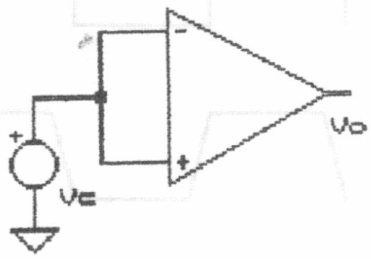
\includegraphics[width=0.4\linewidth]{_fig/op-amp_rrmc-a.png}
		\label{fig:op-amp_rrmc-a}
	}
	\subfloat[modelo]
	{
		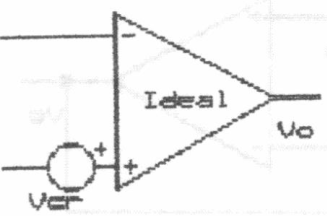
\includegraphics[width=0.4\linewidth]{_fig/op-amp_rrmc-b.png}
		\label{fig:op-amp_rrmc-b}
	}
	\caption{Razón de rechazo de modo común}
	\label{fig:op-amp_rrmc}
\end{figure}

Un amplificador operacional real, con ganancia diferencial $Av$, que tuviera $A_{CM} = 0$ necesitaría, para producir esta misma señal de salida, una señal de entrada $V_{CR}$ que debe satisfacer la relación:

\begin{equation}
	V_{CR} = \frac{Vo}{Av} = \frac{A_{CM} * Vc}{Av} = \frac{Vc}{\text{RRMC}} \quad \text{donde } \text{RRMC} = \left|\frac{Av}{A_{CM}}\right|
\end{equation}

El modelo de la figura \ref{fig:op-amp_rrmc-b} incluye una fuente $V_{CR}$ en serie con la entrada no inversora de un amplificador operacional ideal para tomar en cuenta el efecto recién descrito. Un amplificador operacional ideal tiene $\text{RRMC} = \infty$.

\textbf{Ejemplo.} El amplificador operacional de la figura 1.30a tiene una RRMC real (finita). Hallar una expresión para la tensión de salida, Vo.

En el circuito de la figura \ref{fig:op-amp_ejm9_a}, $V^- = V^+ = Vs$. Así, en este circuito, la señal de modo común es:

\begin{equation}
	Vc = \frac{V^+ + V^-}{2} = Vs
\end{equation}

\begin{figure}[h]
	\centering
	\subfloat[Amplificador no inversor]
	{
		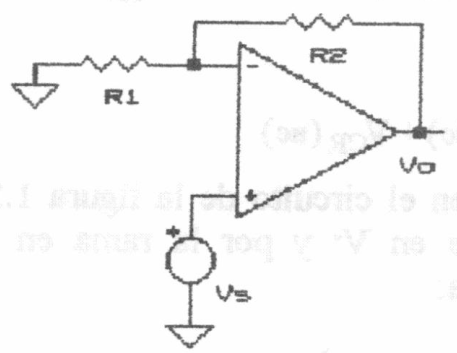
\includegraphics[width=0.4\linewidth]{_fig/op-amp_ejm9_a.png}
		\label{fig:op-amp_ejm9_a}
	}
	\subfloat[circuito equivalente para RRMC finita]
	{
		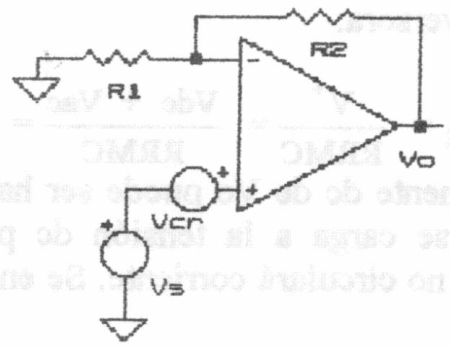
\includegraphics[width=0.4\linewidth]{_fig/op-amp_ejm9_b.png}
		\label{fig:op-amp_ejm9_b}
	}
	\caption{Ejemplo RRMC}
	\label{fig:op-amp_ejm9}
\end{figure}

La señal de salida del circuito equivalente será:

\begin{equation}
	Vo = \left(1 + \frac{R_2}{R_1}\right) * \left(1 + \frac{1}{\text{RRMC}}\right) * Vs
\end{equation}

En la hoja de datos del amplificador operacional se publica valores para $\text{RRMC(dB)}$. Se define $\text{RRMC(dB)} = 20 \log|\text{RRMC}|$. A modo de ejemplo, un amplificador tipo uA741 tiene $\text{RRMC(dB)} = 90\text{ dB}$ (valor típico). Esto corresponde a $|\text{RRMC}| = 31600$.

\begin{figure}[h]
	\centering
	\subfloat[Circuito del ejemplo]
	{
		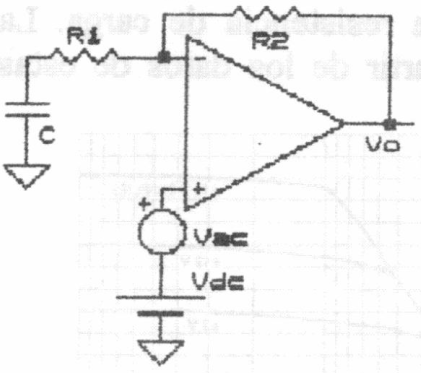
\includegraphics[width=0.3\linewidth]{_fig/op-amp_ejm9_c1.png}
		\label{fig:op-amp_ejm9_c1}
	}
	\subfloat[Circuito para las componentes $DC$ de $Vo$]
	{
		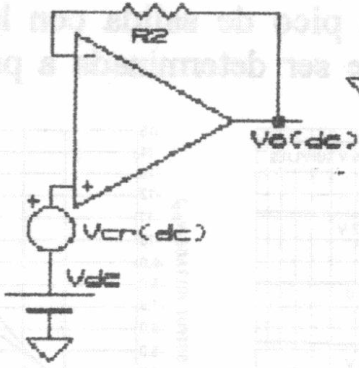
\includegraphics[width=0.3\linewidth]{_fig/op-amp_ejm9_c2.png}
		\label{fig:op-amp_ejm9_c2}
	}
	\subfloat[Circuito para las componentes $AC$ de $Vo$]
	{
		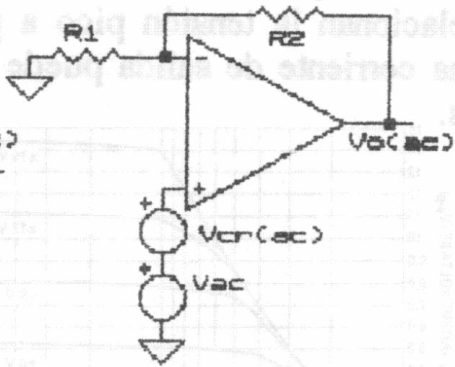
\includegraphics[width=0.3\linewidth]{_fig/op-amp_ejm9_c3.png}
		\label{fig:op-amp_ejm9_c3}
	}
	\caption{Tensión de desbalance de entradas, $V_{OS}$}
	\label{fig:op-amp_ejm9b}
\end{figure}

\textbf{Ejemplo.} En el circuito de la figura \ref{fig:op-amp_ejm9_c1}, la tensión de modo común es:

\begin{equation}
	V^+ = V^- = Vdc + Vac
\end{equation}

El efecto de la razón de rechazo de modo común finita del amplificador operacional se considera agregando, en este caso, una fuente $V_{CR}$ en serie con la entrada inversora:

\begin{equation}
	V_{CR} = \frac{V^+}{\text{RRMC}} = \frac{Vdc + Vac}{\text{RRMC}} = V_{CR}(\text{dc}) + V_{CR}(\text{ac})
\end{equation}

La componente dc de $Vo$ puede ser hallada en el circuito de la figura 1.30Ab. El capacitor se carga a la tensión dc presente en $V^-$ y por la rama en que está conectado no circulará corriente. Se encuentra:

\begin{equation}
	Vo(\text{dc}) = Vdc + V_{CR}(\text{dc}) = Vdc \left(1 + \frac{1}{\text{RRMC}}\right)
\end{equation}

El circuito para la componente ac de $Vo$ se muestra en la figura 1.30Ac. Se supone que el capacitor se comporta como un cortocircuito para la señal:

\begin{equation}
	Vo(\text{ac}) = (Vac + V_{CR}(\text{ac})) \left(1 + \frac{R_2}{R_1}\right) = Vac \left(1 + \frac{R_2}{R_1}\right) \left(1 + \frac{1}{\text{RRMC}}\right)
\end{equation}

La tensión de salida total es:

\begin{equation}
	Vo = Vo(\text{dc}) + Vo(\text{ac})
\end{equation}

\subsection{Máxima corriente en el terminal de salida}
La hoja de datos incluye el valor de corriente de cortocircuito que puede suministrar el terminal de salida del amplificador operacional. Además, frecuentemente los fabricantes incluyen curvas que relacionan la tensión pico a pico de salida con la resistencia de carga. La máxima corriente de salida puede ser determinada a partir de los datos de estas curvas.

\begin{figure}[h]
	\centering
	\subfloat[Excursión positiva]
	{
		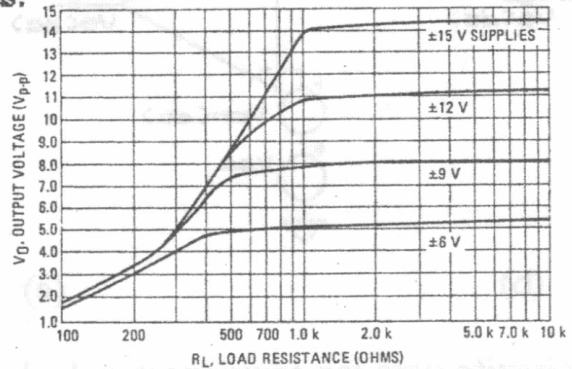
\includegraphics[width=0.4\linewidth]{_fig/op-amp_mcts_tp-a.png}
		\label{fig:op-amp_mcts_tp-a}
	}
	\subfloat[Excursión negativa]
	{
		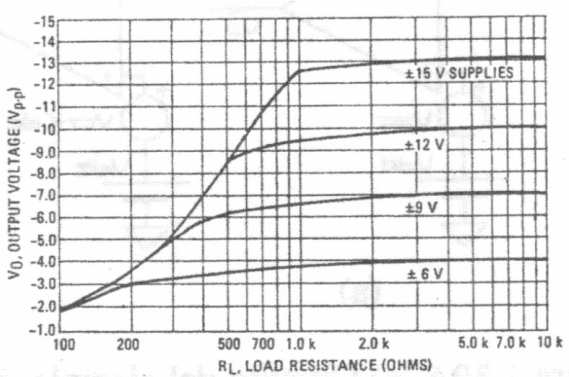
\includegraphics[width=0.4\linewidth]{_fig/op-amp_mcts_tp-b.png}
		\label{fig:op-amp_mcts_tp-b}
	}
	\caption{Variación de la tensión pico de salida con la resistencia de carga}
	\label{fig:op-amp_mcts_tp}
\end{figure}

\section{Amplificadores operacionales retroalimentados por corriente}
En los últimos años han aparecido los llamados amplificadores operacionales realimentados por corriente (AORC) que tienen una estructura diferente a la de un amplificador operacional convencional. El símbolo y el circuito equivalente de este tipo de amplificadores se muestra en la figura \ref{fig:op-amp_aorc-a}.

\begin{figure}[h]
	\centering
	\subfloat[Símbolo]
	{
		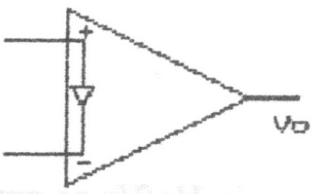
\includegraphics[width=0.4\linewidth]{_fig/op-amp_aorc_simbolo.png}
		\label{fig:op-amp_aorc_simbolo}
	}
	\subfloat[Circuito equivalente]
	{
		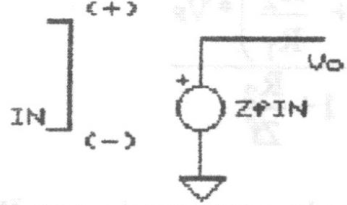
\includegraphics[width=0.4\linewidth]{_fig/op-amp_aorc_eq1.png}
		\label{fig:op-amp_aorc_eq1}
	}
	\caption{Amplificador operacional realimentado por corriente}
	\label{fig:op-amp_aorc-a}
\end{figure}

En estos amplificadores la impedancia entre las entradas es muy baja por lo que la tensión en ambas entradas es aproximadamente la misma. Por su parte, la tensión de salida depende de la corriente $I_N$ en la entrada inversora, en la forma indicada en la figura \ref{fig:op-amp_aorc_eq1}.

En la figura \ref{fig:op-amp_aorc-b} se muestra la implementación de un amplificador no inversor usando un amplificador operacional realimentado por corriente y su circuito equivalente.

\begin{figure}[h]
	\centering
	\subfloat[Símbolo]
	{
		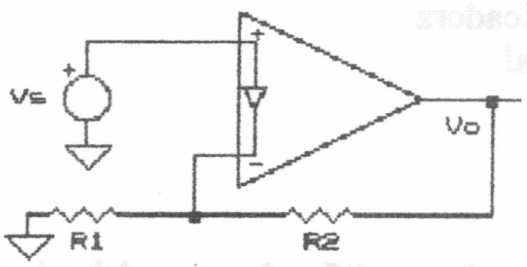
\includegraphics[width=0.4\linewidth]{_fig/op-amp_aorc_sch.png}
		\label{fig:op-amp_aorc_sch}
	}
	\subfloat[Circuito equivalente]
	{
		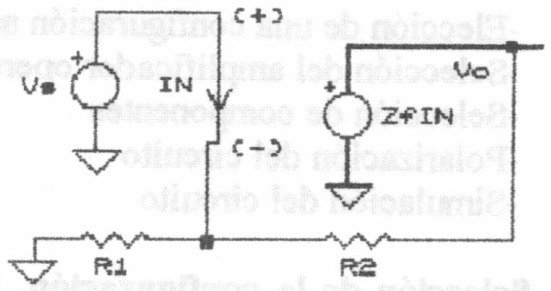
\includegraphics[width=0.4\linewidth]{_fig/op-amp_aorc_eq2.png}
		\label{fig:op-amp_aorc_eq2}
	}
	\caption{Amplificador operacional realimentado por corriente}
	\label{fig:op-amp_aorc-b}
\end{figure}

En el circuito de la figura \ref{fig:op-amp_aorc_eq2} se verifica que:

\begin{equation}
	I_N = \frac{Vs}{R_1||R_2} - \frac{Vo}{R_2}
\end{equation}

\begin{equation}
	Vo = Zf * I_N
\end{equation}

Así:

\begin{equation}
	Vo = \frac{\left(1 + \dfrac{R_2}{R_1}\right) * Vs}{1 + \dfrac{R_2}{Zf}}
\end{equation}

Si $Zf$ es muy grande comparado con $R_2$ la ganancia $Vo/Vs$ se aproxima a la de un amplificador no inversor implementado con un amplificador operacional convencional. La transimpedancia $Zf$ es una función de la frecuencia en la forma: $Zf = Zo / (1 + jf/f_H)$, lo cual afecta la ganancia de tensión $Vo/Vs$ a valores elevados de frecuencia. Sin embargo, en este tipo de amplificadores y a diferencia de los amplificadores operacionales convencionales, existe cierta libertad para fijar la ganancia de voltaje en forma relativamente independiente de la frecuencia de corte.

\section{Consideraciones de diseño}
Amplificadores operacionales convencionales. En esta sección, se tratan ciertos aspectos básicos del diseño de amplificadores simples basados en amplificadores operacionales.

El diseño de un amplificador incluye los siguientes aspectos:

\begin{itemize}
	\item Elección de una configuración amplificadora
	\item Selección del amplificador operacional
	\item Selección de componentes
	\item Polarización del circuito
	\item Simulación del circuito
\end{itemize}

\subsection{Selección dela configuración}
El tipo de amplificador que deberá usarse depende de las características de la señal de entrada. Si la señal de entrada está referida a tierra, se podrá usar una de las configuraciones básicas, esto es, amplificador inversor o amplificador no inversor. Si, en cambio la señal de entrada proviene de una fuente flotante (no conectada a tierra), se deberá recurrir al empleo de amplificadores diferenciales o de instrumentación.

\subsubsection{Amplificador inversor y amplificador no inversor}
Estas estructuras se muestran nuevamente, por comodidad, en la figura \ref{fig:op-amp_single_inv-noinv}.

\begin{figure}[h]
	\centering
	\subfloat[Símbolo]
	{
		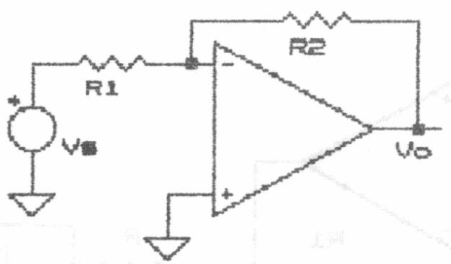
\includegraphics[width=0.4\linewidth]{_fig/op-amp_single_inv.png}
		\label{fig:op-amp_single_inv}
	}
	\subfloat[Circuito equivalente]
	{
		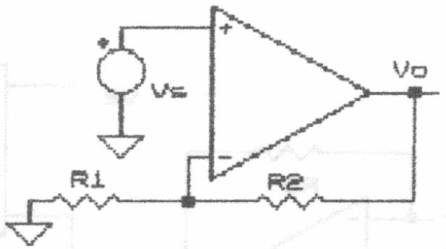
\includegraphics[width=0.4\linewidth]{_fig/op-amp_single_noinv.png}
		\label{fig:op-amp_single_noinv}
	}
	\caption{Amplificador operacional realimentado por corriente}
	\label{fig:op-amp_single_inv-noinv}
\end{figure}

La principal diferencia entre las dos configuraciones está en el nivel de impedancia de entrada. Zi puede alcanzar valores muy elevados en el amplificador no inversor. En cambio, en el amplificador inversor $Zi \cong R_1$. Otra diferencia entre ambas configuraciones es la inversión de fase que ocurre en el amplificador inversor. Probablemente, en la mayor parte de las aplicaciones, este cambio de fase no tiene mayor significación.

Finalmente, el error por razón de rechazo de modo común finita del amplificador operacional y que afecta únicamente al amplificador no inversor, no tiene gran importancia en amplificadores simples.

De acuerdo a lo anterior, la elección de la configuración se basará principalmente en el nivel de impedancia de entrada deseado. En aquellos casos en que el valor de Zi no deba satisfacer ciertas especificaciones se podrá usar indistintamente cualquiera de las dos configuraciones.

\subsubsection{Amplificador diferencial y de instrumentación}
Estos tipos de amplificadores se usan preferentemente en situaciones en que la señal de entrada no está referida a tierra.

La principal diferencia entre los circuitos mostrados en la figura \ref{fig:op-amp_single_diff} y \ref{fig:op-amp_single_instrumentacion} está en el nivel de impedancia de entrada que ambos presentan a la fuente de señal y en el nivel de rechazo de modo común que es mucho más elevado para el amplificador de instrumentación que para el amplificador diferencial. Esta última característica es deseable cuando las líneas que conectan la fuente de señal al amplificador captan interferencia en la forma mostrada en la figura \ref{fig:op-amp_single_misc}. En aplicaciones de alta precisión se deberá optar por el uso de amplificadores de instrumentación integrados.

\begin{figure}[h]
	\centering
	\subfloat[Amplificador diferencial]
	{
		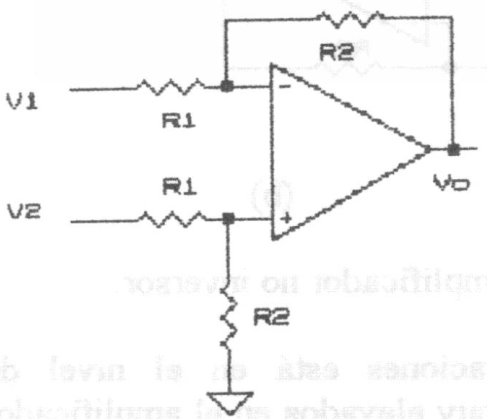
\includegraphics[width=0.3\linewidth]{_fig/op-amp_single_diff.png}
		\label{fig:op-amp_single_diff}
	}
	\subfloat[Amplificador de instrumentación]
	{
		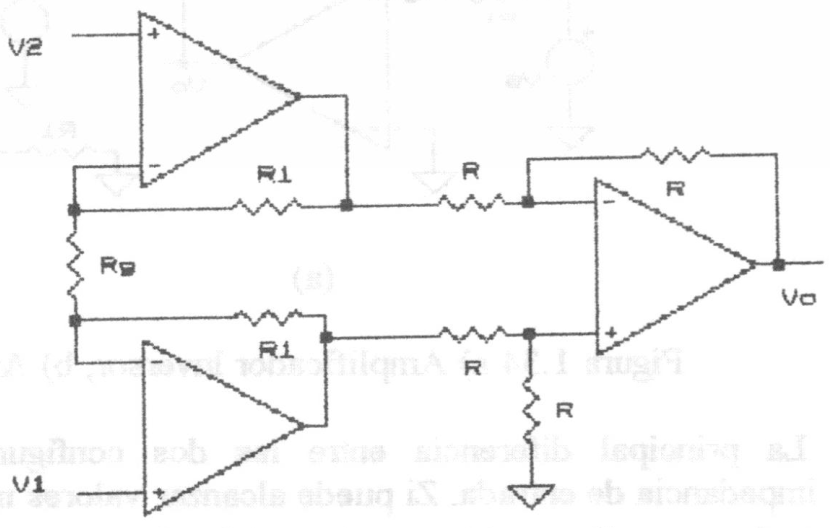
\includegraphics[width=0.3\linewidth]{_fig/op-amp_single_instrumentacion.png}
		\label{fig:op-amp_single_instrumentacion}
	}
	\subfloat[Interferencia de modo común]
	{
		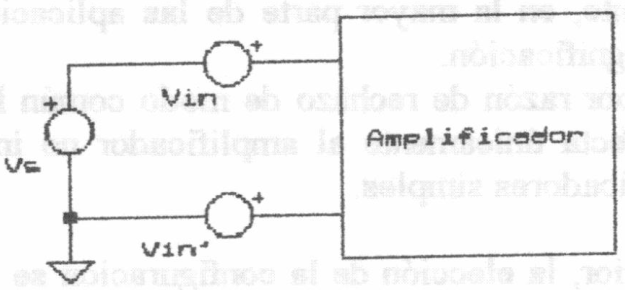
\includegraphics[width=0.3\linewidth]{_fig/op-amp_single_mcomun.png}
		\label{fig:op-amp_single_mcomun}
	}
	\caption{Tensión de desbalance de entradas, $V_{OS}$}
	\label{fig:op-amp_single_misc}
\end{figure}

\subsection{Selección del amplificador operacional}
Los amplificadores operacionales pueden agruparze en las siguientes categorías:
\begin{itemize}
	\item amplificadores de propósitos generales (bajo costo).
	\item amplificadores de gran ancho de banda (alta velocidad).
	\item amplificadores de precisión.
	\item amplificadores de alto voltaje y/o alta corriente de salida.
\end{itemize}

Esta sección está orientada a aplicaciones simples por lo que se supone que la elección del amplificador operacional estará restringida únicamente a dispositivos de propósitos generales. En general, los amplificadores de este grupo tienen ganancias mínimas en lazo abierto del orden de 20000, tensiones de desbalance del orden de 1 mV. Su corriente de polarización en las entradas depende del proceso de fabricación. Algunas características de dispositivos pertenecientes a este grupo de amplificadores operacionales se muestran en la siguiente tabla.

\textbf{Características de algunos amplificadores operacionales de propósitos generales.}

\begin{center}
	\begin{tabular}{lccccc}
		\textbf{Amplif.} & \textbf{$\mathbf{dV_{OS}/dT}$ (uV/$^\circ$C)} & \textbf{$\mathbf{I_b}$ (nA)} & \textbf{$\mathbf{f_T}$ (MHz)} & \textbf{CMRR (dB)} & \textbf{Avo} \\
		& \textbf{(máximo)} & \textbf{(máximo)} & \textbf{(típico)} & \textbf{(mínimo)} & \textbf{(mínimo)} \\
		301A (No comp) & 30 & 500 & 1.0 & 70 & 25000 \\
		324A (quad) & 30 & 250 & 1.0 & 65 & 25000 \\
		355 (FET) & - & 0.2 & 2.5 & 80 & 25000 \\
		741C (Comp) & - & 500 & 1.2 & 70 & 20000 \\
		3140 (MOSFET) & - & 0.04 & 4.0 & 80 & 20000
	\end{tabular}
\end{center}

Comp: Compensado; No comp: no compensado; quad: 4 amplificadores en una pastilla.

Las principales diferencias entre los amplificadores de la tabla anterior están en la magnitud de la corriente de polarización de las entradas, el producto ganancia*ancho de banda ($f_T$) y la razón de rechazo de modo común (RRMC).

\subsection{Selección de los componentes amplificador inversor}
\textbf{Amplificador inversor.} En este circuito, mostrado en la figura 1.36a, la tensión de salida está dada idealmente por:

\begin{equation}
	Vo = - \frac{R_2}{R_1} * Vs
\end{equation}

En la práctica, la señal de salida es:

\begin{equation}
	Vo = - \frac{R_2}{R_1} * Vs - \left(1 + \frac{R_2}{R_1}\right) * V_{OS} - \left(I_B - \frac{I_{OS}}{2}\right) * R_2
\end{equation}

donde $V_{OS}$ es la tensión de desbalance de las entradas, $I_B$ es la corriente de polarización de las entradas e $I_{OS}$ es la corriente de desbalance de las entradas. $V_{OS}$, $I_B$ e $I_{OS}$ dependen de la temperatura interna del amplificador operacional y, en condiciones normales de operación, varían muy lentamente.

En la ecuación anterior se observa que:

\begin{itemize}
	\item La ganancia de tensión es $K = \frac{Vo}{Vs} = - \frac{R_2}{R_1}$.
\end{itemize}

\begin{figure}[h]
	\centering
	\subfloat[Amplificador inversor]
	{
		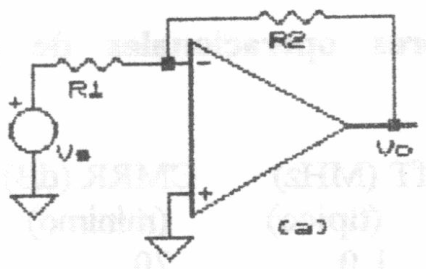
\includegraphics[width=0.3\linewidth]{_fig/op-amp_single_inv2.png}
		\label{fig:op-amp_single_inv2}
	}
	\subfloat[Reducción del efecto de $V_{OS}$ mediante un capacitor en serie con $R_1$]
	{
		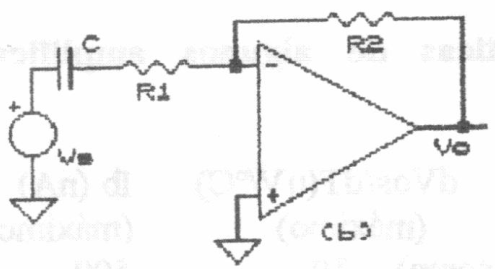
\includegraphics[width=0.3\linewidth]{_fig/op-amp_single_inv-vos.png}
		\label{fig:op-amp_single_inv-vos}
	}
	\subfloat[Cancelación de $I_B$ mediante una resistencia ($R_3$)]
	{
		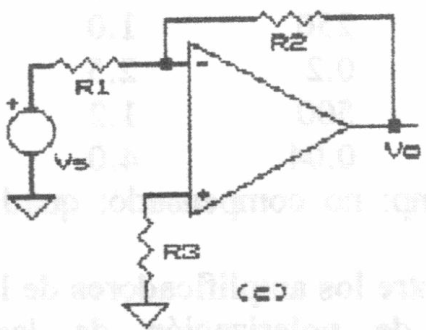
\includegraphics[width=0.3\linewidth]{_fig/op-amp_single_inv-r3.png}
		\label{fig:op-amp_single_inv-r3}
	}
	\caption{Vario, operacionales }
	\label{fig:op-amp_single_misc2}
\end{figure}

\begin{itemize}
	\item El efecto de $V_{OS}$ en la salida aumenta con la magnitud de la ganancia. Sin embargo y tal como se expuso en la sección ???, algunos amplificadores operacionales (741C, 301, etc) disponen de terminales a los que puede conectarse potenciómetros que permiten reducir el valor efectivo de $V_{OS}$. Esta posibilidad no existe en otros amplificadores (324A). Alternativamente, si la señal de entrada no contiene componentes con frecuencias muy bajas, se puede incluir un capacitor en serie con $R_1$ (figura \ref{fig:op-amp_single_inv-vos}) con lo que la ganancia para $V_{OS}$ tendrá una magnitud unitaria. Debe cumplirse que $X_C \ll R_1$.
	\item Por su parte, la magnitud del error producido por $I_B - I_{OS}/2$ puede ser reducida disminuyendo el valor de $R_2$ a un valor tal que el término producido por estas corrientes tome una magnitud aceptable. Si, por ejemplo, se usa un amplificador operacional 741C para implementar el amplificador inversor y se desea que el desplazamiento producido en la salida por $I_B$ no exceda $0.1\text{ volt}$, $R_2$ no podrá exceder $0.1 / (500\text{ nA}) = 200\text{ K}\Omega$. En aplicaciones de mayor precisión puede agregarse una resistencia $R_3$ en serie con la entrada no inversora para anular el efecto de $I_B$. Debe cumplirse que $R_3 = R_1 \,||\, R_2$. En este caso, la componente de error es ahora $I_{OS} R_2 / 2$ en vez de $(I_B - I_{OS}/2) R_2$. Por lo general, $I_B$ es bastante mayor que $I_{OS}$ y esto reduce la magnitud del error.
	\item Otro factor que debe ser considerado en el diseño del amplificador es que, en operación lineal, en ningún instante debe excederse la capacidad de corriente de la salida del amplificador operacional, $Io(\text{máx})$. En el circuito de la figura 1.36a, por ejemplo, la corriente de salida es $Vs/R_1$ y deberá que cumplirse:
\end{itemize}

\begin{equation}
	\frac{Vs(\text{máx})}{R_1} < Io(\text{máx})
\end{equation}

En amplificadores que tengan cargas resistivas conectadas a su salida debe considerarse también la corriente tomada por esas resistencias.

\begin{figure}[h]
	\centering
	\subfloat[Voltaje de salida pico a pico máximo]
	{
		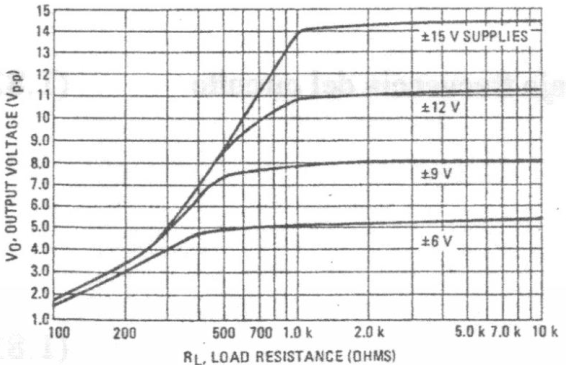
\includegraphics[width=0.4\linewidth]{_fig/op-amp_741_graph-vo-max.png}
		\label{fig:op-amp_741_graph-vo-max}
	}
	\subfloat[Voltaje de salida en función de la resistencia de carga]
	{
		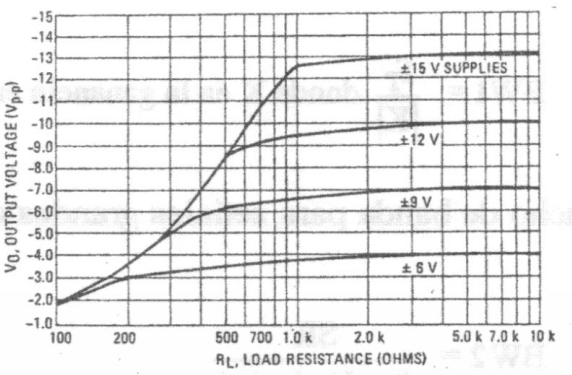
\includegraphics[width=0.4\linewidth]{_fig/op-amp_741_graph-vo-rl.png}
		\label{fig:op-amp_741_graph-vo-rl}
	}
	\caption{Amplificador operacional 741}
	\label{fig:op-amp_741_graph}
\end{figure}

\subsection{Polarización del circuito}
Las fuentes de polarización $\pm V_{CC}$ deben ser elegidas de modo que la salida del amplificador operacional sea capaz de manejar una señal de salida acorde con los requisitos de la aplicación (figura \ref{fig:op-amp_741_graph-vo-max}). Además, la máxima corriente de salida depende de la tensión de polarizaciones (figura \ref{fig:op-amp_741_graph-vo-rl}). En efecto, $Io(\text{máx})$ depende de la magnitud de la tensión de salida y del valor de las fuentes usadas para polarizar el amplificador operacional. Su valor típico puede ser estimado en la curva "Output Voltage Swing as a Function of the Load Resistance", incluída en las hojas de especificaciones del amplificador operacional y mostrada en la figura \ref{fig:op-amp_mcts_tp} y \ref{fig:op-amp_741_graph}.

La corriente de salida pico es:

\begin{equation}
	Io(\text{máx}) = \frac{Vo}{R_L}
\end{equation}

Por ejemplo, si la resistencia vista desde la salida ($R_L$) es de $200\text{ ohm}$ y $\text{Vcc} = \pm 15\text{ volt}$, la tensión de salida no podrá exceder $7\text{ volt}$ (pico a pico). La corriente pico de salida máxima es de:

\begin{equation}
	Io(\text{máx}) = \frac{7/2}{200} = 17.5\text{ mA}
\end{equation}

Este valor corresponde aproximadamente al valor de corriente de cortocircuito que el amplificador operacional es capaz de entregar. Si, en cambio, la resistencia vista desde la salida es de $5\text{ Kohm}$, la máxima tensión de salida es de $27\text{ volt}$ pico a pico o $13.5\text{ volt}$ pico. Esto corresponde a una corriente pico de salida $Io(\text{máx})$ de $2.7\text{ mA}$.

El ancho de banda de pequeña señal del circuito puede ser estimado usando:

\begin{equation}
	\text{BW1} = \frac{f_T}{|K|} \quad \text{donde } K \text{ es la ganancia en baja frecuencia del circuito}
\end{equation}

El ancho de banda para señales grandes es:

\begin{equation}
	\text{BW2} = \frac{\text{SR}}{2\pi Vo(\text{máx})}
\end{equation}

\subsection{Simulación}
El circuito anterior debe simularse mediante algún programa de ayuda al diseño antes de su montaje en laboratorio. En la simulación frecuentemente se detectan errores de diseño.

\textbf{Ejemplo.} Se desea diseñar un amplificador inversor que proporcione una ganancia Kv de $-100$ empleando un amplificador operacional 741 con $V_{OS} = 2\text{ mV}$ e $I_B = 500\text{ nA}$. La tensión de salida tendrá una magnitud máxima de $20\text{ volt}$ pico a pico. Determinar $R_1$ y $R_2$.

De la figura \ref{fig:op-amp_741_graph}, con $Vo = 20\text{ volt}$ (pico a pico), se obtiene $R_L(\text{mín}) = 400\text{ ohm}$ para $\text{Vcc} = 15\text{ volt}$. Esto corresponde a una corriente de salida de $25\text{ mA}$. La corriente total tomada por elementos conectados a la salida (carga, red de realimentación) no podrá exceder este valor.

Si se acepta un desplazamiento de la salida de $50\text{ mV}$ por efectos de $I_B$ se tendrá:

\begin{equation}
	R_2 = \frac{0.050}{500\text{ nA}} = 100\text{ K}\Omega
\end{equation}

La resistencia $R_1$ debe satisfacer la condición de ganancia:

\begin{equation}
	R_1 = \frac{R_2}{|Kv|} = \frac{100\text{ K}\Omega}{100} = 1\text{ K}\Omega
\end{equation}

Se observa que la corriente tomada del terminal de salida tendrá una amplitud $Io(\text{máx})$ dada por:

\begin{equation}
	Io(\text{máx}) = \frac{Vs(\text{máx})}{R_1} = \frac{Vo(\text{máx})}{|Kv| R_1}
\end{equation}

En nuestro problema:

\begin{equation}
	Io(\text{máx}) = \frac{10}{100 * 1\text{ K}} = 100\text{ uA}
\end{equation}

Esta corriente está muy por debajo de la capacidad del amplificador operacional.

La tensión de desbalance, $V_{OS}$, producirá un desequilibrio en la salida de $(1 + Kv) * V_{OS} = 202\text{ mV}$. Este efecto puede disminuirse colocando un capacitor en serie con $R_1$. En este caso la contribución de $V_{OS}$ a la salida bajará a $2\text{ mV}$. La reactancia del capacitor deberá ser pequeña comparada con $R_1$ a la más baja frecuencia de operación.

Dado que el amplificador operacional tiene un producto ganancia ancho de banda de $1.2\text{ MHz}$ y un slew rate de $0.5\text{ volt/us}$, (valores típicos), el circuito tendrá, típicamente, un ancho de banda de pequeña señal de $12\text{ Khz}$ y de gran señal de $8\text{ KHz}$.

El circuito anterior fué simulado mediante PSPICE. Se usó un modelo típico para el amplificador operacional comprobándose que satisface los requisitos del diseño.

El diseño de otros tipos de amplificadores puede realizarse siguiendo un procedimiento similar.	% Amplificadores Operacionales
	\chapter{Diodos}
\section{Generalidades}
???
\subsection{Símbolo y características}
???
\subsection{Resistencia dinámica del diodo}
???
\subsection{Circuito básico}
???
\subsection{Método gráfico}
???
\subsection{Método numérico}
???
\section{Modelos del diodo}
\subsection{Diodo ideal}
???
\subsection{Diodo ideal y fuerte}
???
\subsection{Diodo ideal, fuente $V_f$ y resistencia en serie}
???
\subsection{Diodo Zener}
???
\subsubsection{Símbolo y característica $V/I$}
???
\subsubsection{Modelo del diodo Zener}
???
\section{Aplicaciones de los diodos}
???
\subsection{Circuito recortadores}
???
\subsection{Recordador de dos niveles}
???
\subsection{Circuitos recortadores con amplificadores operacionales}
???
\section{Fuentes de poder}
???
\subsection{Circuito rectificador de media onda}
???
\subsubsection{Corriente media}
???
\subsubsection{Corriente eficaz y potencia disipada}
???
\subsubsection{Regulación}
???
\subsubsection{Máxima tensión inversa $VIP$}
???
\subsection{Rectificador de onda completa}
???
\subsubsection{Corriente media $IDC$}
???
\subsubsection{Valor eficaz de la corriente $IRMS$}
???
\subsubsection{Factor de rizado $FR$}
???
\subsubsection{Regulación $r$}
???
\subsubsection{Máxima tensión inversa}
???
\subsection{Puente rectificador}
???
\subsubsection{Corriente media $IDC$}
???
\subsubsection{Valor eficaz de la corriente $IRMS$}
???
\subsubsection{Factor de rizado $FR$}
???
\subsubsection{Regulación $r$}
???
\subsubsection{Máxima tensión inversa $VIP$}
???
\section{Reducción del factor de rizado}
???
\subsection{Filtro capacitivo}
???
\subsection{Resistencia del secundario del transformador despreciable}
???
\subsubsection{Tensión y corriente continua en las cargas}
???
\subsubsection{Corriente pico en el diodo}
???
\subsubsection{Factor de rizado}
???
\subsubsection{Regulación $r$}
???
\subsubsection{Voltaje inverso máximo $VIP$}
???
\subsection{Resistencia del secundario del transformador no despreciable}
???
\section{Diseño de fuentes de poder}
???
\section{Regulador de tensión con diodos Zener}
???	% Diodos
	\chapter{Transistores Bipolares (BJT)}
\section{Generalidades}
???
\subsection{Símbolos}
???
\subsection{Corrientes y tensiones}
???
\section{Transistores NPN}
???
\subsection{Modelos de operación}
???
\subsection{Operación de un transistor NPN en modo normal}
???
\subsubsection{Curvas características}
???
\subsubsection{Relaciones teóricas}
???
\subsection{Operación de un transistor en continua}
???
\subsubsection{Solución gráfica}
???
\subsubsection{Modelos del transistor de corriente continua}
???
\subsubsection{Puntos de operación, punto de reposo o punto Q}
???
\subsection{Circuitos de polarización en región negativa}
???
\subsubsection{Circuito de polarización fija}
???
\subsubsection{Circuito de auto-polarizado}
???
\section{Transistores PNP}
???
\subsection{Curvas características del transistor PNP}
???
\subsection{Modelos del transistor PNP en corriente continua}
???
\section{Amplificadores con transistores}
???
\subsection{Configuración emisor común}
???
\subsection{Amplificador base común}
???
\subsection{Amplificador colector común}
???
\subsection{Amplificador emisor común con $R_E$}
???
\section{Máxima señal de salida sin distorsión. Rectas de carga}
???
\subsection{Amplificador simple emisor común}
???
\subsubsection{Rectas de carga}
???
\subsubsection{Distorsión}
???
\subsubsection{Magnitud de la máxima señal de salida sin distorsión}
???
\subsubsection{Punto $Q$ óptimo}
???
\subsection{Amplificador con carga acoplada capacitivamente}
???
\subsubsection{Rectas de carga en $DC$}
???
\subsubsection{Recta de carga en alterna}
???
\subsubsection{Magnitud de la máxima señal de salida}
???
\subsection{Otras configuraciones}
???
\subsubsection{Amplificador emisor común con $R_s$}
???
\subsubsection{Amplificador base común}
???
\subsubsection{Amplificador emisor común con $CE$ y carga acoplada capacitivamente}
???
\subsection{Diseño de amplificadores con transistores}
???	% Transistores Bipolares
	% Licencia y derechos: consulte ../../LICENSE-CC-BY-4.0.
% Las figuras y demás materiales de terceros pueden tener derechos separados y deben identificarse.

\chapter{Transistores de Efecto de Campo}
\section{Generalidades}
???
\section{JFET}
\subsection{Símbolo}
???
\subsection{Corriente y tensiones}
???
\section{JFET canal N}
???
\subsection{Curvas características}
???
\subsection{JFET canal N con excitación DC}
???
\subsection{Circuito de polarización}
???
\subsubsection{Circuito de polarización fija}
???
\subsubsection{Auto-polarización}
???
\subsubsection{Polarización compuesta}
???
\subsection{Modelo de señal pequeña}
???
\subsection{Respuesta total}
???
\section{JFET canal P}
???
\subsection{JFET canal P con excitación $DC$}
???
\subsection{Circuito de polarización}
???
\subsection{Modelo de señal}
???
\section{Aplicaciones JFET}
???
\subsection{Amplificador fuente común}
???
\subsection{Amplificador puerto común}
???
\subsection{Amplificador drenador común}
???
\section{Transistores de efecto de campo de metal-oxido semiconductor}
???
\subsection{MOSFET de agotamiento}
???
\subsubsection{Aplicaciones del MOSFET de agotamiento}
???
\subsection{MOSFET de ensanchamiento}
???
\subsubsection{Curvas características de salida}
???
\subsubsection{Circuitos de polarización}
???
\subsubsection{Modelos de señal de MOSFET de ensanchamiento}
???
\subsection{Aplicaciones}
???
\subsubsection{Amplificadores}
???
\subsubsection{Implementación de resistencias controladas por voltaje mediante MOSFET ($VCR$)}
???
\section{Conmutación de potencia}
???
\subsection{Transistores bipolares de puerta aislada}
???
\section{Consideraciones de diseño de amplificadores de tensión con FET}
???	% Transistores de Efecto de Campo
    \chapter{Amplificadores diferenciales y comparadores}
\section{Amplificadores diferenciales}
???
\subsection{Señal de entrada diferencial}
???
\subsection{Señal de entrada de modo común}
???
\subsection{Uso de superposición}
???
\subsection{Razón de rechazo de modo común $RRMC$}
???
\section{Amplificadores diferenciales con transistores}
???
\subsection{Amplificador diferencial básico}
???
\subsubsection{Punto de operación}
???
\subsubsection{Circuito equivalente en AC}
???
\subsubsection{Señal de entrada diferencial}
???
\subsubsection{Señal de entrada en modo común}
???
\subsection{Amplificador diferencial con transistores y $R_E$}
???
\subsubsection{Señal de entrada de modo común}
???
\subsubsection{Señal diferencial de entrada}
???
\subsubsection{Razón de rechazo de modo común}
???
\subsubsection{Impedancia de entrada $Z_{id}$, $Z_{ic}$}
???
\section{Teorema de bisección}
???
\subsection{Excitación simétrica o de modo común}
???
\subsection{Excitación antisimétrica o diferencial}
???
\subsection{Aplicación del teorema de bisección a un amplificador}
???
\subsubsection{Señal de entrada de modo común}
???
\subsubsection{Señal diferencial de entrada}
???
\subsection{Uso de una fuente de corriente en emisor}
???
\subsubsection{Fuente de corriente compensada térmicamente}
???
\subsubsection{Espejo de corriente}
???
\subsection{Amplificador diferencial práctico con transistores}
???
\subsection{Amplificador diferencial con JFET}
???
\section{Comparadores}
???
\subsection{Estructura de la etapa de salida de comparadores}
???
\subsection{Aplicaciones}
???
\subsubsection{Detector de nivel}
???
\subsubsection{Circuito de alarma}
???
\subsection{Efecto del ruido}
???
\subsection{Uso de histéresis en comparadores}
???
\subsubsection{Características de transferencia}
???
\subsubsection{Circuito comparador implementado con comparador tipo colector abierto}
???
\subsection{Amplificador operacional como comparador}
???
\subsection{Selección del comparador}
???
\subsection{Montaje del comparador}
???
\subsection{Características de algunos comparadores}
???
	% Amplificador Diferencial0
		
\end{document}
